\documentclass[12pt]{article}

\pagestyle{headings}

\newenvironment{packed}{\begin{list}{$\bullet$}{\parsep0in\itemsep0in}}{\end{list}}

\usepackage{epsf}

\usepackage{latexsym}

\usepackage{ulem}
\normalem

%
% Macros for specific types of entities.
%
\newcommand{\cmd}[1]{{\em #1}}
\newcommand{\option}[1]{{\em #1}}
\newcommand{\path}[1]{{\bf #1}}
\newcommand{\url}[1]{{\bf #1}}
\newcommand{\xqt}[1]{{\bf #1}}

\textheight=8.50in
\voffset=-.55in
\voffset=-.75in

\setlength{\textwidth}{6.5in}
\setlength{\oddsidemargin}{0in}

\setcounter{secnumdepth}{4}
\setcounter{tocdepth}{2}

\parindent0em
\parskip0.65em

\hyphenation{dns-sec DNS-SEC}
\hyphenation{dns-sec--tools}

%%%%%%%%%%%%%%%%%%%%%%%%%%%%%%%%%%%%%%%%%%%%%%%%%%%%%%%%%%%%%%%%%%%%%%%%%%%%%%

\begin{document}
\markboth{Step-by-Step DNS Security Operator Guidance Document - version 0.5}{Step-by-Step DNS Security Operator Guidance Document - version 0.5}

\begin{titlepage}

\vspace{.5in}

\begin{center}
\LARGE{\bf
SOFTWARE USER MANUAL (SUM):
TRAINING, PROCEDURAL, AND
DEVELOPMENT DOCUMENTATION
}
\vspace{.5in}

\Large{
Step-by-Step DNS Security\\
Operator Guidance Document\\
(Version 1.0)}\\
$[${\it Using the BIND-9.3.0 (or later) distribution}$]$
\vspace{0.5in}

% \Large{
% {\bf Contract: FA8750-04-C-0229
% \vspace{0.125in}
% 
% CDRL A006}\\}
\vspace{2in}
1 December 2006
\end{center}

\vspace{.5in}

SUBMITTED BY

Sparta, Inc\\
7075 Samuel Morse Dr.\\
Columbia, MD 21046-3401
\vspace{0.25in}

% \begin{tabular}{lll}
% 	& Principal Investigator	& Contract/Financial Contact\\
% Name	& George R. Mundy		& Kim Morrill\\
% Phone	& (410) 872-1515		& (410) 872-1515\\
% Fax	& (410) 872-8079		& (410) 872-8079\\
% Email	& Russ.Mundy@sparta.com		& Kim.Morrill@sparta.com\\
% \end{tabular}

\end{titlepage}
\markboth{Step-by-Step DNS Security Operator Guidance Document - version 0.5}{Step-by-Step DNS Security Operator Guidance Document - version 0.5}

%%%%%%%%%%%%%%%%%%%%%%%%%%%%%%%%%%%%%%%%%%%%%%%%%%%%%%%%%%%%%%%%%%%%%%%%%%%%%%

\begin{center}
{\Large
{\bf DNSSEC-Tools\\
Is your domain secure?}}
\end{center}
\tableofcontents
\clearpage
\listoffigures

%%%%%%%%%%%%%%%%%%%%%%%%%%%%%%%%%%%%%%%%%%%%%%%%%%%%%%%%%%%%%%%%%%%%%%%%%%%%%%

\clearpage

\markboth{Step-by-Step DNS Security Operator Guidance Document - version 0.5}{Step-by-Step DNS Security Operator Guidance Document - version 0.5}
\section{Introduction}
\markboth{Step-by-Step DNS Security Operator Guidance Document - version 0.5}{Step-by-Step DNS Security Operator Guidance Document - version 0.5}
\label{intro}


DNS Security (DNSSEC) helps protect against DNS-spoofing attacks by providing
origin authentication and integrity protection of DNS information.  Proper
maintenance of a DNSSEC-enhanced DNS zone is essential to protecting the
domain's zone data.

% This Step-by-Step DNS Security Operator Guidance document is intended for
% operations using the BIND-9.3.0 (or later) distribution [4].  It will assist
% operators in gaining operational experience with DNSSEC. Some basic
% understanding of DNSSEC terms and concepts is required. A good introduction
% to DNSSEC can be found in [5].  Some basic understanding of public key
% cryptography is also required [7].

This Step-by-Step DNS Security Operator Guidance document is intended for
operations using the BIND-9.3.0 (or later) distribution.  It will assist
operators in gaining operational experience with DNSSEC. Some basic
understanding of DNSSEC terms and concepts is required.

This document is meant to be a learning aid and is not intended
to define policy in any form. Any implicit recommendations for key sizes,
signature validity periods, and command line parameters are for illustration
purposes ONLY and MUST NOT be used in production environments unless
due-diligence has been taken to ensure that these values are acceptable within
such environments.  See [1] for suggestions on determining appropriate
security characteristics.

This document was written as part of the DNSSEC-Tools project.  The goal of
this project is to create a set of documentation, tools, patches,
applications, wrappers, extensions, and plug-ins that will help ease the
deployment of DNSSEC-related technologies.  For more information about this
project and the tools that are being developed and provided, please see the
DNSSEC-Tools project web page at:

\url{http://www.dnssec-tools.org}

%%%%%%%%%%%%%%%%%%%%%%%%%%%%%%%%%%%%%%%%%%%%%%%%

\subsection{Organization of this Document}

The following operations are described in this document:

\begin{description}

\item [Section~\ref{preliminaries}] {Essential Preliminaries}\\
This section contains essential instructions that must be followed before
continuing with the rest of the document.

\item [Section~\ref{genzsk}] {Zone-Signing Key (ZSK) Generation}\\
This section describes the procedure for creating new Zone Signing Keys; i.e.,
the keys used for signing zone data.

\item [Section~\ref{genksk}] {Key-Signing Key (KSK) Generation}\\
This section describes the procedure for creating new Key Signing Keys; i.e.,
keys that are used to sign the ZSKs in the apex keyset.

\item [Section~\ref{config-n-serve}] {Configuring and Serving a Signed Zone}\\
This section describes the procedure for serving a signed zone file.

\item [Section~\ref{roll-curzsk}] {Current ZSK Roll-Over}\\
This section describes the procedure for rolling over an old ZSK. These steps
should be used only if the older ZSK is known to have not been compromised.

\item [Section~\ref{roll-ksk}] {KSK Roll-Over}\\
This section describes the procedure for rolling over an old KSK. These steps
should be used only if the older KSK is known to have not been compromised.

\item [Section~\ref{signzone-nodel}] {Signing a Zone with No Delegations}\\
This section describes the procedure for signing a zone that has no
delegations (no non-authoritative NS records) present in the zone file.

\item [Section~\ref{delegation-child}] {Creating a Signed Delegation in a Child Zone}\\
This section describes the activities that a child zone must perform
in order to facilitate the creation of a signed delegation at the parent.

\item [Section~\ref{signzone-hasdel}] {Signing a Zone that Has Delegations}\\
This section describes the procedure for signing a zone that has delegations
(non-authoritative NS records) present in the zone file. The difference
between this and section 3 lies in the additional communication involved
between the parent and the child, as well as creation of the DS record in the
parent zone, when delegations are present.

\item [Section~\ref{delegation-parent}] {Creating a Signed Delegation in a Parent Zone}\\
This section describes the activities that a parent zone must perform
in order to facilitate the creation of a signed delegation at the parent.

\item [Section~\ref{roll-emergency-ksk}] {KSK Roll-Over -- KSK Compromise}\\
This section describes the procedure for performing an emergency roll-over
of the KSK when it is suspected or known to be compromised.

\item [Section~\ref{roll-emergency-curzsk}] {ZSK Roll-Over -- Current ZSK Compromise}\\
This section describes the procedure for performing an emergency roll-over
of the Current ZSK, when it is suspected or known to be compromised.

\item [Section~\ref{roll-emergency-pubzsk}] {ZSK Roll-Over -- Published ZSK Compromise}\\
This section describes the procedure for performing an emergency roll-over
of the Published ZSK, when it is suspected or known to be compromised.

\item [Section~\ref{roll-emergency-zsks}] {ZSK Roll-Over -- Published and Current ZSK Compromise}\\
This section describes the procedure for performing an emergency roll-over
of the Published and Current ZSKs, when both are suspected or known to be
compromised.

\item [Section~\ref{roll-emergency-parent-ksk}] {KSK Roll-Over -- Parent Action During KSK Compromise}\\
This section describes the actions that the parent zone must perform when it
receives notification from the child about a KSK compromise, and before it
publishes a DS value that points to the new KSK in the child.

\end{description}

These sections are followed by several appendices.  These appendices contain
useful information, such as checklists for the operations and pictorial
illustrations for each of the operations described in this guide.

%%%%%%%%%%%%%%%%%%%%%%%%%%%%%%%%%%%%%%%%%%%%%%%%

\subsection{Identifying Relevant Steps}

The following table summarizes the list of steps relevant to different kinds
of zones. The columns marked with an 'X' for any row correspond to those
operations with which the zone operator for that type of zone must be
familiar.

\begin{center}
\begin{tabular}{|l|c|c|c|c|c|c|c|c|c|c|c|c|c|c|}
\hline
{\bf Zone Profile} & \multicolumn{14}{c|}{{\bf Steps}} \\
\cline{2-15}
 & 1 & 2 & 3 & 4 & 5 & 6 & 7 & 8 & 9 & 10 & 11 & 12 & 13 & 14 \\
\hline
No signed delegations, & X & X & X &   & X &   &   & X & X & X & X & X & X & \\
parent is not signed   &   &   &   &   &   &   &   &   &   &   &   &   &   & \\
\hline
No signed delegations, & X & X & X &   & X & X &   & X & X & X & X & X & X & \\
parent is signed       &   &   &   &   &   &   &   &   &   &   &   &   &   & \\
\hline
Signed delegations,    & X & X &   & X & X &   & X & X & X & X & X & X & X & X\\
parent is not signed   &   &   &   &   &   &   &   &   &   &   &   &   &   &  \\
\hline
Signed delegations,    & X & X &   & X & X & X & X & X & X & X & X & X & X & X\\
parent is signed       &   &   &   &   &   &   &   &   &   &   &   &   &   &  \\
\hline
\end{tabular}
\end{center}

%%%%%%%%%%%%%%%%%%%%%%%%%%%%%%%%%%%%%%%%%%%%%%%%

\subsection{Key Concepts}
\begin{description}
\item{ZSK} - Zone-Signing Key\\
The key used to sign zone data.

\item{KSK} - Key-Signing Key\\
The key used to sign the ZSKs in the apex keyset.

\item{Current ZSK}\\
The Current ZSK is the key that is currently used to sign zone data.

\item{Published ZSK}\\
The Published ZSK is the key that is pre-published in the zone file as the
future ZSK.

\item{New ZSK}\\
The New ZSK is the key that is scheduled to become the Published ZSK.

\end{description}

%%%%%%%%%%%%%%%%%%%%%%%%%%%%%%%%%%%%%%%%%%%%%%%%

\subsection{Conventions Used in this Document}

One of the goals of this document is to self-contain DNS Security
operations within sections and prevent constant cross-referencing between
sections.  Consequently, certain parts of the text are repeated throughout
the document.

In particular, one might notice that zone SOA serial numbers may not change
between sections.  This should {\bf not} be taken as an indication that the
serial numbers do not need to change when the guide states that they should.

Text marked in bold represents text or commands entered by users
within a given procedural step.

Underlined text, which can also be in bold, is a place-holder for actual
run-time values.  These values are either automatically generated or are
values that are known to the user from some other step.

Additionally, the following typographical conventions are used in this
document.

\begin{tabular}{lll}
\cmd{command}		& & Command names\\
\path{path}		& & File and path names\\
\url{URL}		& & Web URLs\\
\xqt{execution}		& & Simple command executions\\
\end{tabular}

Longer sets of command sequences are given in this format:
\begin{tabbing}
\hspace{0.5in}\$ {\bf cd /tmp} $[$ENTER$]$ \\
\hspace{0.5in}\$ {\bf ls} $[$ENTER$]$ \\
\hspace{0.5in}\$ {\bf rm -fr *} $[$ENTER$]$ \\
\hspace{0.5in}\$ \\
\end{tabbing}

In most cases, output will not be displayed for given command sequences.

%%%%%%%%%%%%%%%%%%%%%%%%%%%%%%%%%%%%%%%%%%%%%%%%

\subsection{Acknowledgments}

This document builds upon the procedures described in [1] for key
roll-over techniques; the step-by-step instructions described in
Sections~\ref{roll-curzsk} and~\ref{roll-ksk} are meant to closely follow
the recommendations given by that document. Early versions of this guide
were reviewed and critiqued by SAIC, Inc./Quotient, Inc., including Rip
Loomis and Rob Payne.  Their contributions are much appreciated.

%%%%%%%%%%%%%%%%%%%%%%%%%%%%%%%%%%%%%%%%%%%%%%%%

\subsection{Comments}

Please send any comments and corrections to developers@dnssec-tools.org.



%%%%%%%%%%%%%%%%%%%%%%%%%%%%%%%%%%%%%%%%%%%%%%%%%%%%%%%%%%%%%%%%%%%%%%%%%%%%%%

\clearpage

\markboth{Step-by-Step DNS Security Operator Guidance Document - version 0.5}{Step-by-Step DNS Security Operator Guidance Document - version 0.5}
\section{Essential Preliminaries}
\markboth{Step-by-Step DNS Security Operator Guidance Document - version 0.5}{Step-by-Step DNS Security Operator Guidance Document - version 0.5}
\label{preliminaries}

The following sections must be read before proceeding with the rest of this
guide.

The steps in Sections~\ref{check-random} and~\ref{check-bind} {\bf MUST} be
taken prior to following any other steps.  Section~\ref{zone-serials}'s
discussion of this guides use of zone file serial numbers {\bf MUST} be
understood prior to following any other steps.  Failure to do any of these
three could affect the security of your zone.

Section~\ref{key-tags-tables} describes {\it key-tags} tables, which are used
to manage DNSSEC information about encryption keys and signed zones.  This
section should be understood prior to reading the remainder of the document.

%%%%%%%%%%%%%%%%%%%%%%%%%%%%%%%%%%%%%%

\subsection{Check for Randomness}
\label{check-random}

Key generation and zone signing require random data to create strong
cryptographic material.  The \cmd{dnssec-keygen} and \cmd{dnssec-signzone}
commands default to using random data from \path{/dev/random}.  Use this test
to verify that \path{/dev/random} will provide data when requested:

\begin{tabbing}
\hspace{0.5in} \= 12345678 \= 12345678 \= 12345678 \= 12345678 \kill \\
\hspace{0.5in}\$ {\bf dd if=/dev/random bs=2 count=10 $|$ od -x} $[$ENTER$]$ \\
\hspace{0.5in}...\\
\hspace{0.5in}\$ \\
\end{tabbing}

The above command checks if \path{/dev/random} is able to provide random data
when queried; it does not check to see that the data provided is truly random.

If this command provides data immediately, then \path{/dev/random} will
provide the data you need.  If it hangs, then \cmd{dnssec-keygen} and
\cmd{dnssec-signzone} won't be able to retrieve random data from
\path{/dev/random}.

% If this check for randomness fails, pseudorandom numbers can be used instead
% [6].  However, using pseudorandom numbers significantly affects the quality
% of the crypto material.  A more appropriate measure would be to run the
% key-generation and zone-signing operations on a different system that has
% \path{/dev/random} and the ability to generate good random data [2].

If this check for randomness fails, pseudorandom numbers can be used instead.
However, using pseudorandom numbers significantly affects the quality
of the crypto material.  A more appropriate measure would be to run the
key-generation and zone-signing operations on a different system that has
\path{/dev/random} and the ability to generate good random data.

%%%%%%%%%%%%%%%%%%%%%%%%%%%%%%%%%%%%%%

\clearpage
\subsection{Check for Correct Version of BIND}
\label{check-bind}

BIND version 9.3.0 (or later) is {\bf required} for use with this document.
Before following any of these instructions, you {\bf must} ensure that you
have the correct version of BIND.

The BIND version may be verified by checking the version of
\cmd{dnssec-keygen}:

\begin{tabbing}
\hspace{0.5in} \= 12345678 \= 12345678 \= 12345678 \= 12345678 \kill \\
\hspace{0.5in} \$ {\bf dnssec-keygen -h} $[$ENTER$]$ \\
\hspace{0.5in} Usage: \\
\hspace{0.5in} \>dnssec-keygen -a alg -b bits -n type [options] name \\
\hspace{0.5in} Version: 9.3.0 \\
\hspace{0.5in} ...... \\
\hspace{0.5in} \$
\end{tabbing}

If the version is incorrect, you must install the correct version of BIND
before proceeding.

%%%%%%%%%%%%%%%%%%%%%%%%%%%%%%%%%%%%%%

\subsection{Zone File Serial Numbers}
\label{zone-serials}

This guide contains a number of instructions to update a zone file.  In each,
it is indicated that the zone file's serial number must be updated.  The
actual serial numbers used will depend on each installation's preferred method
of using serial numbers.  The method used in this document is YYYYMMDDNN,
where:
\begin{packed}
\item {\bf YYYY} - year
\item {\bf MM} - month
\item {\bf DD} - day
\item {\bf NN} - incrementing number
\end{packed}

For example, the third zone file change on January 9, 2005, would be given
as 2005090103.

The serial numbers used in this guide are {\it generally} increasing
throughout the document.  More importantly, however, the numbers used within
each section are {\it always} increasing.

Some sections of this guide direct you to perform steps in other sections.
Regardless of the serial numbers given in these steps, your zone file's serial
numbers {\bf must} increase with each modification or your changes will not
be seen.

%%%%%%%%%%%%%%%%%%%%%%%%%%%%%%%%%%%%%%%%%%%%%%%%

\clearpage
\subsection{Key-Tags Tables}
\label{key-tags-tables}

Data about results of the different steps described in this document must be
retained for use in other steps.  These data include such things as the names
of generated keys, key status, and the date a zone was signed.  While these
data may be kept in whatever form an administrator finds most convenient,
this guide stores them in a {\it key-tags table}.

A key-tags table stores a zone name, the zone's ZSK keys, the zone's KSK keys,
and the zone's expiration date.  The following is a template of how the
key-tags table is used in this document.  Data about the zone's KSK, Current
ZSK, Published ZSK, and New ZSK are stored here:

\begin{center}
\begin{tabular}{|c|c|c|c|c|c|c|c|c|c|}
\hline
{\bf Zone} &
\multicolumn{4}{c|}{{\bf ZSK}} &
\multicolumn{4}{c|}{{\bf KSK}} &
{\bf Exp} \\
\cline{2-9}

 & Tag & Size & Creat & S & Tag & Size & Creat & S & \\
\hline

			&
\underline{zsktag-cur}	&
512			&
\underline{date}	&
C			&
\underline{ksktag}	&
1024			&
\underline{date}	&
C			& \\

\cline{2-9}

\underline{zone.name}	&
\underline{zsktag-pub}	&
512			&
\underline{date}	&
P			&
& & & & \\

			&
\underline{zsktag-new}	&
512			&
\underline{date}	&
N			&
& & & & \\

\hline
\end{tabular}
\end{center}

The {\it -cur}, {\it -pub}, and {\it -new} suffixes used in this key-tags
table and in the rest of this guide are used for illustration purposes only.
They are not intended to be used in the key-tags table for an operational
zone.  Similarly, for convenience and identification purposes the tags are
retained with particular keys even when the status changes.

The following is an example key-tags table containing non-template data.
There are entries for two zones:  {\it example.com} and {\it example.net}.
There are entries for a example.com's Current KSK, New KSK, Current ZSK,
Published ZSK, and New ZSK.  example.net's entries are for its Current KSK,
Current ZSK, and Published ZSK.

\begin{center}
\begin{tabular}{|c|c|c|c|c|c|c|c|c|c|}
\hline
{\bf Zone} &
\multicolumn{4}{c|}{{\bf ZSK}} &
\multicolumn{4}{c|}{{\bf KSK}} &
{\bf Exp} \\
\cline{2-9}

 & Tag & Size & Creat & S & Tag & Size & Creat & S & \\
\hline

			&
32267	&
512			&
8/15/05	&
C			&
65037	&
1024			&
9/21/04	&
C			& \\

\cline{2-9}

example.com		&
40379	&
512			&
8/20/05	&
P			&
14895	&
1024			&
9/21/05	&
N			&
9/21/05			\\

\cline{2-9}

			&
58406	&
512			&
8/25/05	&
N			&
& & & & \\

\hline

example.net		&
30449	&
512			&
7/24/05	&
C			&
25384	&
1024			&
1/09/05	&
C			&
9/27/05			\\

\cline{2-9}

			&
38715	&
512			&
8/27/05	&
P			&
& & & & \\

\hline

\end{tabular}
\end{center}

As stated above, this information may be kept in whatever form each
administrator finds convenient.  Some administrators may want to have separate
key-tags tables for each zone for which they are responsible; others may wish
to maintain all their zones in a single table.

A blank template key-tags table may be found in Appendix~\ref{app-keytags}.
Additional versions (PostScript, Excel spreadsheet) may be found on
\url{http://www.dnssec-tools.org}.

%%%%%%%%%%%%%%%%%%%%%%%%%%%%%%%%%%%%%%%%%%%%%%%%%%%%%%%%%%%%%%%%%%%%%%%%%%%%%%

\clearpage

\markboth{Step-by-Step DNS Security Operator Guidance Document - version 0.5}{Step-by-Step DNS Security Operator Guidance Document - version 0.5}
\section{Normal Operations for All Zones}
\markboth{Step-by-Step DNS Security Operator Guidance Document - version 0.5}{Step-by-Step DNS Security Operator Guidance Document - version 0.5}
\label{normal-all}

This section describes those normal DNSSEC operations which are relevant for
all zones.  These operations are:

\begin{itemize}
\item Zone-Signing Key (ZSK) Generation
\item Key-Signing Key (KSK) Generation
\item Configuring and Serving a Signed Zone
\item Current ZSK Roll-Over
\item KSK Roll-Over
\end{itemize}


\clearpage
\subsection{Zone-Signing Key (ZSK) Generation}
\label{genzsk}

This section provides the steps required to generate a new Zey-Signing Key   
(ZSK).  See Figure~\ref{fig:keygen}.

%%%%%%%%%%%%%%%%%%%%%%%%%%%%%%%%%%%%%%


\subsubsection{Generate the Key}

Use the \cmd{dnssec-keygen} command to generate a key 512 bits long. 
\begin{tabbing}
\hspace{0.5in} \= 12345678 \= 12345678 \= 12345678 \= 12345678 \kill
\hspace{0.5in}\$ {\bf dnssec-keygen -a RSASHA1 -b 512 -n ZONE \underline{zone.name}} \\
\hspace{0.5in} [ENTER] \\
\hspace{0.5in} K\underline{zone.name}.+005+\underline{zsktag} \\
\hspace{0.5in}\$ \\
\end{tabbing}

The process may take a few minutes to return its results. If the process
appears to have stalled, run the command using a pseudo-random number
generator as follows:
\begin{tabbing}
\hspace{0.5in} \= 12345678 \= 12345678 \= 12345678 \= 12345678 \kill \\
\hspace{0.5in}\$ {\bf dnssec-keygen -r /dev/urandom -a RSASHA1 -b 512} \\
\hspace{0.5in} {\bf -n ZONE \underline{zone.name}} [ENTER] \\
\hspace{0.5in} K\underline{zone.name}.+005+\underline{zsktag} \\
\hspace{0.5in}\$ \\
\end{tabbing}

Two files are output by \cmd{dnssec-keygen}: \\
    - Private key contained in \path{K\underline{zone.name}.+005+\underline{zsktag}.private}\\
    - Public key contained in \path{K\underline{zone.name}.+005+\underline{zsktag}.key}

{\bf \underline{zone.name}} - the name of the zone (e.g., example.com)\\
{\bf \underline{zsktag}} - the key identifier (e.g., 57011) 

You must note this number in the key-tag table as you walk through this
document.  This number is automatically generated and should not be changed.
The key id will be the only field in the filename that changes as you rotate
keys, so it must be tracked.

This document uses RSASHA1 as the cryptographic algorithm, which is
represented by the ``005'' in the key name's algorithm field.



%%%%%%%%%%%%%%%%%%%%%%%%%%%%%%%%%%%%%%

\subsubsection{Update the Key-Tags Table}

Keep a record of the key-tags that currently refer to ZSKs.

\begin{center}
\begin{tabular}{|c|c|c|c|c|c|c|c|c|c|}
\hline
{\bf Zone} &
\multicolumn{4}{c|}{{\bf ZSK}} &
\multicolumn{4}{c|}{{\bf KSK}} &
{\bf Exp} \\
\cline{2-9}

 & Tag & Size & Creat & S & Tag & Size & Creat & S & \\
\hline

\underline{zone.name} & \underline{zsktag} & 512 & \underline{date} & & & & & & \\

\hline
\end{tabular}
\end{center}

Leave the status field (S) empty for now.

%%%%%%%%%%%%%%%%%%%%%%%%%%%%%%%%%%%%%%


\subsubsection{Store Separately the Private Keys for ZSKs and KSKs}

Storing the private keys for ZSKs and KSKs off-line is considered a good
security practice.  ZSK and KSK separation lessens the operational burden
during zone-key compromise, but only if the KSK is still considered safe for
use.  In cases where a signed zone is also updated via dynamic updates, the
ZSK will need to be on-line and available to the name server process.  To
avoid a common vulnerability point (such as compromise of the system on which
these keys reside), store the KSKs in a place that is considered safer.





\clearpage
\subsection{Key-Signing Key (KSK) Generation}
\label{genksk}

This section provides the steps required to generate a new Key-Signing Key
(KSK).  See Figure~\ref{fig:keygen}.

%%%%%%%%%%%%%%%%%%%%%%%%%%%%%%%%%%%%%%

\subsubsection{Generate the Key}

Use the \cmd{dnssec-keygen} command to generate a key 1024 bits long.  Key
size is a rough measure of strength; KSKs are generally made stronger than
ZSKs.

\begin{tabbing}
\hspace{0.5in} \= 12345678 \= 12345678 \= 12345678 \= 12345678 \kill \\
\hspace{0.5in} \$ {\bf dnssec-keygen -a RSASHA1 -b 1024 -n ZONE -f KSK} {\bf \underline{zone.name}} \\
\hspace{0.5in} [ENTER] \\
\hspace{0.5in} K\underline{zone.name}.+005+\underline{ksktag} \\
\hspace{0.5in} \$ \\
\end{tabbing}

The process may take a few minutes to return its results. If the process
appears to have stalled, run the command using a pseudo-random number
generator as follows:

\begin{tabbing}
\hspace{0.5in} \= 12345678 \= 12345678 \= 12345678 \= 12345678 \kill \\
\hspace{0.5in} \$ {\bf dnssec-keygen -r /dev/urandom -a RSASHA1 -b 1024 -n ZONE -f KSK} \\
\hspace{0.5in} {\bf \underline{zone.name}} [ENTER] \\
\hspace{0.5in} K\underline{zone.name}.+005+\underline{ksktag} \\
\hspace{0.5in} \$ \\
\end{tabbing}

Two files are output by \cmd{dnssec-keygen}: \\
    - Private key contained in \path{K\underline{zone.name}.+005+\underline{ksktag}.private}\\
    - Public key contained in \path{K\underline{zone.name}.+005+\underline{ksktag}.key}

{\bf \underline{zone.name}} - the name of the zone (e.g., example.com)\\
{\bf \underline{ksktag}} - the key identifier (e.g., 24818) 

You must note this number in the key-tag table as you walk through this
document.  This number is automatically generated and should not be changed.
The key id will be the only field in the filename that changes as you rotate
keys, so it must be tracked.

This document uses RSASHA1 as the cryptographic algorithm, which is
represented by the ``005'' in the key name's algorithm field.

%%%%%%%%%%%%%%%%%%%%%%%%%%%%%%%%%%%%%%

\subsubsection{Update the Key-Tags Table}

Keep a record of the key-tags that currently refer to KSKs.

\begin{center}
\begin{tabular}{|c|c|c|c|c|c|c|c|c|c|}
\hline
{\bf Zone} &
\multicolumn{4}{c|}{{\bf ZSK}} &
\multicolumn{4}{c|}{{\bf KSK}} &
{\bf Exp} \\
\cline{2-9}

 & Tag & Size & Creat & S & Tag & Size & Creat & S & \\
\hline

\underline{zone.name} & & & & & \underline{ksktag} & 1024 & \underline{date} & & \\

\hline
\end{tabular}
\end{center}

Leave the status field (S) empty for now.

%%%%%%%%%%%%%%%%%%%%%%%%%%%%%%%%%%%%%%


\subsubsection{Store Separately the Private Keys for ZSKs and KSKs}

Storing the private keys for ZSKs and KSKs off-line is considered a good
security practice.  ZSK and KSK separation lessens the operational burden
during zone-key compromise, but only if the KSK is still considered safe for
use.  In cases where a signed zone is also updated via dynamic updates, the
ZSK will need to be on-line and available to the name server process.  To
avoid a common vulnerability point (such as compromise of the system on which
these keys reside), store the KSKs in a place that is considered safer.





\clearpage
\subsection{Configuring and Serving a Signed Zone}
\label{config-n-serve}

Several configuration files must be modified in order to serve a signed zone.
Follow the steps below to configure your name server and have it start
serving your signed zone.

\path{named.conf} is the name of the configuration file used in these examples.
The configuration file may vary according to the needs of the administrator.

%%%%%%%%%%%%%%%%%%%%%%%%%%%%%%%%%%%%%%

\subsubsection{Add the Signed Zone to the Name Server Configuration File}

The name of the signed zone file must be added to the name server's
configuration file.  For the zone whose name is \underline{zone.name},
do the following:
\begin{tabbing}
\hspace{0.5in} \= 12345678 \= 12345678 \= 12345678 \= 12345678 \kill \\
\hspace{0.5in}\$ {\bf vi named.conf} $[$ENTER$]$ \\
\hspace{0.5in} ... \\
\hspace{0.5in} zone "\underline{zone.name}." \{ \\
\hspace{0.5in} \> \> type master; \\
\hspace{0.5in} \> \> file "\underline{zonefile}.signed"; \\
\hspace{0.5in} \}; \\
\hspace{0.5in} ... \\
\hspace{0.5in}\$ \\
\end{tabbing}

%%%%%%%%%%%%%%%%%%%%%%%%%%%%%%%%%%%%%%

\subsubsection{Enable DNSSEC}

Add the \option{dnssec-enable yes;} option to the \path{named.conf} file.
\begin{tabbing}
\hspace{0.5in} \= 12345678 \= 12345678 \= \kill \\
\hspace{0.5in}\$ {\bf vi named.conf} $[$ENTER$]$ \\
\hspace{0.5in} ... \\
\hspace{0.5in} options \{ \\
\hspace{0.5in} \> \> ... \\
\hspace{0.5in} \> \> dnssec-enable yes; \\
\hspace{0.5in} \}; \\
\hspace{0.5in} ... \\
\hspace{0.5in}\$ \\
\end{tabbing}

%%%%%%%%%%%%%%%%%%%%%%%%%%%%%%%%%%%%%%

\subsubsection{Check the Name Server Configuration File for Errors}

You must ensure that the configuration file modifications were performed
correctly.  The \cmd{named-checkconf} command will perform this verification.
No output indicates that all is well with the zone.

\begin{tabbing}
\hspace{0.5in}\$ {\bf named-checkconf \underline{named.conf}} $[$ENTER$]$ \\
\hspace{0.5in}\$ \\
\end{tabbing}

%%%%%%%%%%%%%%%%%%%%%%%%%%%%%%%%%%%%%%


\subsubsection{Reload the Zone}

The \cmd{rndc} command will reload the name server configuration files and
the zone contents.  The name server process is assumed to be already running.

\begin{tabbing}
\hspace{0.5in}\$ {\bf rndc reload zone.name} $[$ENTER$]$ \\
\hspace{0.5in}\$ \\
\end{tabbing}


%%%%%%%%%%%%%%%%%%%%%%%%%%%%%%%%%%%%%%

\subsubsection{Check that the Zone Loaded Properly}

Confirm that the SOA serial number of the zone corresponds to the most
recent value.

\begin{tabbing}
\hspace{0.5in}\$ {\bf dig @\underline{server-IP-address} SOA \underline{zone.name}} $[$ENTER$]$ \\
\hspace{0.5in} ; $<$$<$$>$$>$ DiG 9.3.0 $<$$<$$>$$>$ ... \\
\hspace{0.5in} ... \\
\hspace{0.5in} ;; flags: qr aa rd; QUERY: 1, ANSWER: 1, AUTHORITY: 1, ADDITIONAL: 0 \\
\hspace{0.5in} ... \\
\hspace{0.5in} ;;ANSWER SECTION \\
\hspace{0.5in} 12345678 \= 12345678 \= 12345678 \= 12345678 \= 12345678 \= 12345678 \= 12345678 \= 12345678 \kill
\hspace{0.5in} \underline{zone.name} \> \> 3600 \> IN \> SOA \> servername contact ( \\
\hspace{0.5in}	\> \> \> \> 2005092101 ; This should be the most  \\
\hspace{0.5in}	\> \> \> \> \> ; recent value. \\
\hspace{0.5in}	\> \> \> \> \> ; This value will most \\
\hspace{0.5in}	\> \> \> \> \> ; likely be different in \\
\hspace{0.5in}	\> \> \> \> \> ; your zone file. \\
\hspace{0.5in}				... \\
\hspace{0.5in} \> ) \\
\hspace{0.5in}... \\
\hspace{0.5in}\$ \\

\end{tabbing}


\clearpage
\subsection{Current ZSK Roll-Over}
\label{roll-curzsk}

This section gives the steps necessary for the pre-publish scheme for ZSK
roll-over.  The alternative, the double-signature method, is used for rolling
over KSKs.  Double signatures for records signed by the ZSK can increase the
size of the zone many times.  The pre-publish scheme, although requiring more
steps for the roll-over, does not suffer from this problem. The size argument
does not apply during KSK roll-over since the DNSKEY RRset is the only record
doubly signed by the KSK.

See Figure~\ref{fig:zskroll}.

%%%%%%%%%%%%%%%%%%%%%%%%%%%%%%%%%%%%%%

\subsubsection{Ensure that Sufficient Time has Elapsed Since the Last Roll-Over}

The time between roll-overs has to be at least twice the maximum zone TTL
period.  This is the largest TTL in the entire zone file multiplied by two.

%%%%%%%%%%%%%%%%%%%%%%%%%%%%%%%%%%%%%%

\subsubsection{Sign Zone with the KSK and Published ZSK}

Follow steps \ref{check-zonefile-unsigned-nodeleg}~--~\ref{signzone-nodel-last}
if the zone does no delegation.  Follow steps
\ref{check-zonefile-unsigned-deleg}~--~\ref{signzone-deleg-last} if the
zone does delegation.  The ZSK used in the signing process in
Section~\ref{signzone-no-deleg} or~\ref{signzone-has-deleg} must be the key
that is marked as the Published key (P) in the key-tag table. The KSK used
as input to \cmd{dnssec-signzone} does not change, so the keyset does not
change and does not have to be re-sent to the parent.

Record the signature expiry date in the key-tag table.

\begin{center}
\begin{tabular}{|c|c|c|c|c|c|c|c|c|c|}
\hline
{\bf Zone} &
\multicolumn{4}{c|}{{\bf ZSK}} &
\multicolumn{4}{c|}{{\bf KSK}} &
{\bf Exp} \\
\cline{2-9}

 & Tag & Size & Creat & S & Tag & Size & Creat & S & \\
\hline

\underline{zone.name}	&
\underline{zsktag-cur}	&
512			&
\underline{date}	&
C			&
\underline{ksktag}	&
1024			&
\underline{date}	&
C			&
\underline{date}	\\

\cline{2-9}

			&
\underline{zsktag-pub}	&
512			&
\underline{date}	&
P			&
& & & & \\

\hline
\end{tabular}
\end{center}

%%%%%%%%%%%%%%%%%%%%%%%%%%%%%%%%%%%%%%


\subsubsection{Reload the Zone}

The \cmd{rndc} command will reload the name server configuration files and
the zone contents.  The name server process is assumed to be already running.

\begin{tabbing}
\hspace{0.5in}\$ {\bf rndc reload zone.name} $[$ENTER$]$ \\
\hspace{0.5in}\$ \\
\end{tabbing}


%%%%%%%%%%%%%%%%%%%%%%%%%%%%%%%%%%%%%%

\subsubsection{Wait for Old Zone Data to Expire from Caches}

Wait at least twice the maximum zone TTL period for the old zone data to
expire from name server caches.  This is the largest TTL in the entire zone
file multiplied by two.  This will also allow the new data to propagate.

%%%%%%%%%%%%%%%%%%%%%%%%%%%%%%%%%%%%%%


\subsubsection{Generate a New ZSK}

Generate a new ZSK, as described in section~\ref{genzsk}.
Update the key-tag table with the new ZSK, and set its status to New (N).

\begin{center}
\begin{tabular}{|c|c|c|c|c|c|c|c|c|c|}
\hline
{\bf Zone} &
\multicolumn{4}{c|}{{\bf ZSK}} &
\multicolumn{4}{c|}{{\bf KSK}} &
{\bf Exp} \\
\cline{2-9}

 & Tag & Size & Creat & S & Tag & Size & Creat & S & \\
\hline

			&
\underline{zsktag-cur}	&
512			&
\underline{date}	&
C			&
\underline{ksktag}	&
1024			&
\underline{date}	&
C			&
			\\

\cline{2-9}

\underline{zone.name}	&
\underline{zsktag-pub}	&
512			&
\underline{date}	&
P			&
& & & & 
\underline{date}	\\

\cline{2-9}

				&
{\bf \underline{zsktag-new}}	&
{\bf 512}			&
{\bf \underline{date}}		&
{\bf N}				&
& & & &	\\

\hline
\end{tabular}
\end{center}



\subsubsection{Modify the Zone File}

The zone file must be modified to account for the key changes.  The Current
ZSK must be deleted and the New ZSK must be added.  Also, the SOA serial
number must be changed so that the zone file's new contents will be recognized.

\begin{tabbing}
\hspace{0.5in} \= 12345678 \= 12345678 \= 12345678\= 12345678 \= 12345678 \kill
\hspace{0.5in}\$ {\bf vi \underline{zonefile}} $[$ENTER$]$ \\
\hspace{0.5in}\underline{zone.name} \> \> \> IN \> SOA \> servername contact (\\
\hspace{3.5in}{\bf 2005092102} ; Increase current value by 1. \\
\hspace{4.4in};  This value may be different \\
\hspace{4.4in}; in your zone file. \\
\hspace{0.5in}\>           \>         ... \\
\hspace{0.5in}\>              ) \\
\hspace{0.5in}... \\
\hspace{0.5in};; ksk \\
\hspace{0.5in}\$INCLUDE ``/path/to/K\underline{zone.name}.+005+\underline{ksktag}.key'' \\
\hspace{0.5in}{\bf \sout{;; cur zsk}} \\
\hspace{0.5in}{\bf \sout{\$INCLUDE ``/path/to/K\underline{zone.name}.+005+\underline{zsktag-cur}.key''}} \\
\hspace{0.5in};; pub zsk \\
\hspace{0.5in}\$INCLUDE ``/path/to/K\underline{zone.name}.+005+\underline{zsktag-pub}.key'' \\
\hspace{0.5in}{\bf ;; new zsk} \\
\hspace{0.5in}{\bf \$INCLUDE ``/path/to/K\underline{zone.name}.+005+\underline{zsktag-new}.key}'' \\
\hspace{0.5in}... \\
\hspace{0.5in}\$ \\
\end{tabbing}


\subsubsection{Update the Key-Tags Table}

Update the key-tags table to reflect the changed key status.  Delete the old
Current ZSK. Change the status of the Published ZSK to Current.  Change the
status of the New ZSK to Published.

\begin{center}
\begin{tabular}{|c|c|c|c|c|c|c|c|c|c|}
\hline
{\bf Zone} &
\multicolumn{4}{c|}{{\bf ZSK}} &
\multicolumn{4}{c|}{{\bf KSK}} &
{\bf Exp} \\
\cline{2-9}

 & Tag & Size & Creat & S & Tag & Size & Creat & S & \\
\hline

					&
{\bf \sout{\underline{zsktag-cur}}}	&
{\bf \sout{512}}			&
{\bf \sout{\underline{date}}}		&
{\bf \sout{C}}				&
\underline{ksktag}			&
1024					&
\underline{date}			&
C					&
					\\

\cline{2-9}

\underline{zone.name}	&
\underline{zsktag-pub}	&
512			&
\underline{date}	&
{\bf \sout{P}}		&
& & & &
\underline{date}			\\

			&
			&
			&
			&
{\bf C}			&
& & & & \\

\cline{2-9}

			&
\underline{zsktag-new}	&
512			&
\underline{date}	&
{\bf \sout{N}}		&
& & & & \\

			&
			&
			&
			&
{\bf P}			&
& & & & \\

\hline
\end{tabular}
\end{center}



%%%%%%%%%%%%%%%%%%%%%%%%%%%%%%%%%%%%%%

\subsubsection{Sign the Zone with the KSK and Current ZSK}

Follow the steps
\ref{check-zonefile-unsigned-nodeleg}~--~\ref{signzone-nodel-last}
if the zone does no delegation.  Follow the steps
\ref{check-zonefile-unsigned-deleg}~--~\ref{signzone-deleg-last}
if the zone does delegation.  The ZSK used in the signing process in
Section~\ref{signzone-no-deleg} or~\ref{signzone-has-deleg} must be the key
that is marked as the Current key (C) in the key-tag table (this was the older
Published key.) The KSK used as input to \cmd{dnssec-signzone} does not
change, so the keyset does not change and does not have to be re-sent to the
parent.


Record the signature expiry date in the key-tag table.

\begin{center}
\begin{tabular}{|c|c|c|c|c|c|c|c|c|c|}
\hline
{\bf Zone} &
\multicolumn{4}{c|}{{\bf ZSK}} &
\multicolumn{4}{c|}{{\bf KSK}} &
{\bf Exp} \\
\cline{2-9}

 & Tag & Size & Creat & S & Tag & Size & Creat & S & \\
\hline

\underline{zone.name}	&
\underline{zsktag-pub}	&
512			&
\underline{date}	&
C			&
\underline{ksktag}	&
1024			&
\underline{date}	&
C			&
\underline{date}	\\

\cline{2-9}

			&
\underline{zsktag-new}	&
512			&
\underline{date}	&
P			&
& & & & \\

\hline
\end{tabular}
\end{center}

%%%%%%%%%%%%%%%%%%%%%%%%%%%%%%%%%%%%%%

\subsubsection{Reload the Zone}

The \cmd{rndc} command will reload the name server configuration files and
the zone contents.  The name server process is assumed to be already running.

\begin{tabbing}
\hspace{0.5in}\$ {\bf rndc reload zone.name} $[$ENTER$]$ \\
\hspace{0.5in}\$ \\
\end{tabbing}


\subsubsection{Dispose of the Old Zone Key}

Delete the old ZSK's {\it .private} and {\it .key} files.



\clearpage
\subsection{KSK Roll-Over}
\label{roll-ksk}

This section gives the steps necessary for the double-signature scheme for
KSK roll-over.  The alternative, the pre-publish method, is used for rolling
over ZSKs.  Double signatures for records signed by the ZSK can increase the
size of the zone many times.  The pre-publish scheme, although requiring more
steps for the roll-over, does not suffer from this problem. The size argument
does not apply during KSK roll-over since the DNSKEY RRset is the only record
doubly signed by the KSK.

See Figure~\ref{fig:kskroll}.

%%%%%%%%%%%%%%%%%%%%%%%%%%%%%%%%%%%%%%

\subsubsection{Ensure that Sufficient Time has Elapsed Since the Last Roll-Over}

The time between roll-overs has to be at least twice the maximum zone TTL
period.  This is the largest TTL in the entire zone file multiplied by two.

%%%%%%%%%%%%%%%%%%%%%%%%%%%%%%%%%%%%%%

\subsubsection{Generate a New KSK}

Generate a new KSK, as described in section~\ref{genksk}.

\begin{center}
\begin{tabular}{|c|c|c|c|c|c|c|c|c|c|}
\hline
{\bf Zone} &
\multicolumn{4}{c|}{{\bf ZSK}} &
\multicolumn{4}{c|}{{\bf KSK}} &
{\bf Exp} \\
\cline{2-9}

 & Tag & Size & Creat & S & Tag & Size & Creat & S & \\
\hline

\underline{zone.name}	&
\underline{zsktag-cur}	&
512			&
\underline{date}	&
C			&
\underline{ksktag}	&
1024			&
\underline{date}	&
C			&
\underline{date}	\\

\cline{2-9}

				&
\underline{zsktag-pub}		&
512				&
\underline{date}		&
P				&
{\bf \underline{ksktag}}	&
{\bf 1024}			&
{\bf \underline{date}}		&
{\bf P}				&
				\\

\hline
\end{tabular}
\end{center}

%%%%%%%%%%%%%%%%%%%%%%%%%%%%%%%%%%%%%%

\subsubsection{Modify the Zone File}

The zone file must be modified to account for the new KSK.  The SOA serial
number also must be changed so that the zone file's new contents will be
recognized.

\begin{tabbing}
\hspace{0.5in} \= 12345678 \= 12345678 \= 12345678 \= 12345678 \kill \\
\hspace{0.5in}\$ {\bf vi \underline{zonefile}} $[$ENTER$]$ \\
\hspace{0.5in}\underline{zone.name}        IN     SOA        servername contact ( \\
\hspace{3.5in}{\bf 2005092103} ; Increase current value by 1. \\
\hspace{4.4in};  This value may be different \\
\hspace{4.4in}; in your zone file. \\
\hspace{0.5in}\>           \>         ... \\
\hspace{0.5in}\>              ) \\
\hspace{0.5in}... \\
\hspace{0.5in};; cur ksk \\
\hspace{0.5in}\$INCLUDE ``/path/to/K\underline{zone.name}.+005+\underline{ksktag}.key'' \\
\hspace{0.5in}{\bf ;; new ksk} \\
\hspace{0.5in}{\bf \$INCLUDE ``/path/to/K\underline{zone.name}.+005+\underline{ksktag-pub}.key}'' \\
\hspace{0.5in};; cur zsk \\
\hspace{0.5in}\$INCLUDE ``/path/to/K\underline{zone.name}.+005+\underline{zsktag-cur}.key'' \\
\hspace{0.5in};; pub zsk \\
\hspace{0.5in}\$INCLUDE ``/path/to/K\underline{zone.name}.+005+\underline{zsktag-pub}.key'' \\
\hspace{0.5in}... \\
\hspace{0.5in}\$ \\
\end{tabbing}

%%%%%%%%%%%%%%%%%%%%%%%%%%%%%%%%%%%%%%


\subsubsection{Re-Sign the Zone DNSKEY RRset with the Current and Published KSK}

ZSKs sign the zone data, whereas KSKs sign the RRset for all DNSKEYs 
recognized by the zone. There is no direct way to create the signed DNSKEY
RRset for the zone; it is only formed as a by-product of the 
\cmd{dnssec-signzone} operation.

Follow steps
\ref{check-zonefile-unsigned-nodeleg}~--~\ref{signzone-nodel-last}
if the zone does no delegation.  Follow steps
\ref{check-zonefile-unsigned-deleg}~--~\ref{signzone-deleg-last}
if the zone does delegation.  The ZSK used in the signing process in
Section~\ref{signzone-no-deleg} or~\ref{signzone-has-deleg} must be the key
that is marked as the Current key (C) in the key-tag table. Both Current KSK
and the Published KSK must be simultaneously included in the
\cmd{dnssec-signzone} operation (by using two \option{-k} options).



Record the signature expiry date in the key-tag table.

\begin{center}
\begin{tabular}{|c|c|c|c|c|c|c|c|c|c|}
\hline
{\bf Zone} &
\multicolumn{4}{c|}{{\bf ZSK}} &
\multicolumn{4}{c|}{{\bf KSK}} &
{\bf Exp} \\
\cline{2-9}

 & Tag & Size & Creat & S & Tag & Size & Creat & S & \\
\hline

\underline{zone.name}		&
\underline{zsktag-cur}		&
512			&
\underline{date}			&
C			&
\underline{ksktag-cur}		&
1024			&
\underline{date}			&
C			&
{\bf\underline{date}}	\\

\cline{2-9}

			&
\underline{zsktag-pub}	&
512			&
\underline{date}	&
P			&
\underline{ksktag-pub}		&
1024			&
\underline{date}			&
P			&
			\\

\hline
\end{tabular}
\end{center}

Although the keyset has changed, it {\bf must not} be sent to the parent yet.

%%%%%%%%%%%%%%%%%%%%%%%%%%%%%%%%%%%%%%


\subsubsection{Reload the Zone}

The \cmd{rndc} command will reload the name server configuration files and
the zone contents.  The name server process is assumed to be already running.

\begin{tabbing}
\hspace{0.5in}\$ {\bf rndc reload zone.name} $[$ENTER$]$ \\
\hspace{0.5in}\$ \\
\end{tabbing}


%%%%%%%%%%%%%%%%%%%%%%%%%%%%%%%%%%%%%%

\subsubsection{Wait for Old DNSKEY RRset to Expire from Caches}

Wait at least twice the maximum zone TTL period for the old DNSKEY RRset to
expire from name server caches.  This is the largest TTL in the entire zone
file multiplied by two.  This will also allow the new data to propagate.

%%%%%%%%%%%%%%%%%%%%%%%%%%%%%%%%%%%%%%

\subsubsection{Modify the Zone File}

The zone file must be modified to account for the key changes.  The Current
ZSK must be deleted and the New ZSK must be added.  Also, the SOA serial
number must be changed so that the zone file's new contents will be recognized.

\begin{tabbing}
\hspace{0.5in} \= 12345678 \= 12345678 \= 12345678 \= 12345678 \kill \\
\hspace{0.5in}\$ {\bf vi \underline{zonefile}} $[$ENTER$]$ \\
\hspace{0.5in}\underline{zone.name}        IN     SOA        servername contact ( \\
\hspace{3.5in}{\bf 2005092104} ; Increase current value by 1. \\
\hspace{4.4in};  This value may be different \\
\hspace{4.4in}; in your zone file. \\
\hspace{0.5in}\>           \>         ... \\
\hspace{0.5in}\>              ) \\
\hspace{0.5in}... \\
\hspace{0.5in}{\bf \sout{;; cur ksk}} \\
\hspace{0.5in}{\bf \sout{\$INCLUDE ``/path/to/K\underline{zone.name}.+005+\underline{ksktag-cur}.key''}} \\
\hspace{0.5in};; new ksk \\
\hspace{0.5in}\$INCLUDE ``/path/to/K\underline{zone.name}.+005+\underline{ksktag-pub}.key'' \\
\hspace{0.5in};; pub zsk \\
\hspace{0.5in}\$INCLUDE ``/path/to/K\underline{zone.name}.+005+\underline{zsktag-pub}.key'' \\
\hspace{0.5in}{\bf ;; new zsk} \\
\hspace{0.5in}{\bf \$INCLUDE ``/path/to/K\underline{zone.name}.+005+\underline{zsktag-new}.key}'' \\
\hspace{0.5in}... \\
\hspace{0.5in}\$ \\
\end{tabbing}

%%%%%%%%%%%%%%%%%%%%%%%%%%%%%%%%%%%%%%


\subsubsection{Re-Sign the Zone DNSKEY RRset with the Current and Published KSK}

ZSKs sign the zone data, whereas KSKs sign the RRset for all DNSKEYs 
recognized by the zone. There is no direct way to create the signed DNSKEY
RRset for the zone; it is only formed as a by-product of the 
\cmd{dnssec-signzone} operation.

Follow steps
\ref{check-zonefile-unsigned-nodeleg}~--~\ref{signzone-nodel-last}
if the zone does no delegation.  Follow steps
\ref{check-zonefile-unsigned-deleg}~--~\ref{signzone-deleg-last}
if the zone does delegation.  The ZSK used in the signing process in
Section~\ref{signzone-no-deleg} or~\ref{signzone-has-deleg} must be the key
that is marked as the Current key (C) in the key-tag table. Both Current KSK
and the Published KSK must be simultaneously included in the
\cmd{dnssec-signzone} operation (by using two \option{-k} options).



%%%%%%%%%%%%%%%%%%%%%%%%%%%%%%%%%%%%%%

\label{kskroll-new-keyset}

%%%%%%%%%%%%%%%%%%%%%%%%%%%%%%%%%%%%%%

\subsubsection{Update the Key-Tags Table with the Latest KSK}

Delete the Current KSK and change the status of the new KSK from Published
(P) to Current (C).  Record the signature expiry date in the key-tag table.

\begin{center}
\begin{tabular}{|c|c|c|c|c|c|c|c|c|c|}
\hline
{\bf Zone} &
\multicolumn{4}{c|}{{\bf ZSK}} &
\multicolumn{4}{c|}{{\bf KSK}} &
{\bf Exp} \\
\cline{2-9}

 & Tag & Size & Creat & S & Tag & Size & Creat & S & \\
\hline

					&
\underline{zsktag-cur}			&
512					&
\underline{date}			&
C					&
{\bf \sout{\underline{ksktag-cur}}}	&
{\bf \sout{1024}}			&
{\bf \sout{\underline{date}}}		&
{\bf \sout{C}}				&
					\\

\cline{2-9}

\underline{zone.name}	&
\underline{zsktag-pub}	&
512			&
\underline{date}	&
P			&
\underline{ksktag-pub}	&
1024			&
\underline{date}	&
{\bf \sout{C}}		&
{\bf\underline{date}}	\\

			&
			&
			&
			&
			&
			&
			&
			&
{\bf P}			&
			\\

\hline
\end{tabular}
\end{center}

%%%%%%%%%%%%%%%%%%%%%%%%%%%%%%%%%%%%%%

\subsubsection{Perform Steps in Section~\ref{delegation-child} if this Zone
is a Secure Delegation from Another Zone}

The keyset generated in~\ref{kskroll-new-keyset} contains only the new KSK.
This keyset must be sent to the parent in order to complete the secure
delegation.

%%%%%%%%%%%%%%%%%%%%%%%%%%%%%%%%%%%%%%


\subsubsection{Reload the Zone}

The \cmd{rndc} command will reload the name server configuration files and
the zone contents.  The name server process is assumed to be already running.

\begin{tabbing}
\hspace{0.5in}\$ {\bf rndc reload zone.name} $[$ENTER$]$ \\
\hspace{0.5in}\$ \\
\end{tabbing}


\subsubsection{Dispose of the Old KSK}

Delete the old KSK's {\it .private} and {\it .key} files.



%%%%%%%%%%%%%%%%%%%%%%%%%%%%%%%%%%%%%%%%%%%%%%%%%%%%%%%%%%%%%%%%%%%%%%%%%%%%%%

\clearpage

\markboth{Step-by-Step DNS Security Operator Guidance Document - version 0.5}{Step-by-Step DNS Security Operator Guidance Document - version 0.5}
\section{Normal Operations for Child Zones}
\markboth{Step-by-Step DNS Security Operator Guidance Document - version 0.5}{Step-by-Step DNS Security Operator Guidance Document - version 0.5}
\label{normal-child}

This section describes those normal DNSSEC operations which are relevant
for child zones.  These operations are:

\begin{itemize}
\item Signing a Zone that Has No Delegations
\item Creating a Signed Delegation in a Child Zone
\end{itemize}


\clearpage
\subsection{Signing a Zone with No Delegations}
\label{signzone-nodel}

A zone needs to be re-signed when \underline{any} change is made to it.
Steps~\ref{keygen-set-nodel} and~\ref{signzone-nodeleg-updzf}
must be followed if the zone has not been previously signed.
Steps~\ref{check-zonefile-unsigned-nodeleg}~-~\ref{signzone-nodel-last}
must be followed when re-signing a zone file that has no
delegations.


\subsubsection{Generate Two ZSKs and One KSK}

Follow the steps in Section~\ref{genzsk} for generating the ZSKs and steps in
Section~\ref{genksk} for generating the KSK.

Designate one of the two ZSKs as the Current (C) zone signing key and use it
to sign the zone data; designate the other as the Published (P) key, which
is for future use following a ZSK roll-over.  Set the status of each of these
keys in the column marked S.

There is only one KSK and this is used to sign the zone apex keyset; mark its
status as Current (C).  The Published ZSK should be kept more
safely\footnote{It would be a good idea for an operator to apply increased
protection mechanisms (physical, file permissions and ownership, network,
etc.) to the Published ZSK than are used for the Current ZSK.}
than the Current ZSK.  The idea is that the Published ZSK can be easily rolled
in even if the Current ZSK is compromised (the Current ZSK may have to be
kept on-line in some circumstances).

If the KSK has been stored in a more secure location (off-line, more highly
protected directory, etc.) then it might be a good idea to store the
Published ZSK in the same secure location.

\begin{center}
\begin{tabular}{|c|c|c|c|c|c|c|c|c|c|}
\hline
{\bf Zone} &
\multicolumn{4}{c|}{{\bf ZSK}} &
\multicolumn{4}{c|}{{\bf KSK}} &
{\bf Exp} \\
\cline{2-9}

 & Tag & Size & Creat & S & Tag & Size & Creat & S & \\
\hline

\underline{zone.name}	&
\underline{zsktag-cur}	&
512			&
\underline{date}	&
C			&
\underline{ksktag}	&
1024			&
\underline{date}	&
C			& \\

\cline{2-9}

			&
\underline{zsktag-pub}	&
512			&
\underline{date}	&
P			&
& & & & \\

\hline
\end{tabular}
\end{center}
		\label{keygen-set-nodel}

\subsubsection{Modify the Zone File}

The zone file must be modified to account for the new keys.  Add lines to
include the KSK and the ZSKs in the zone file.  Also, the SOA serial number
must be changed so that the zone file's new contents will be recognized.

\begin{tabbing}
\hspace{0.5in} \= 12345678 \= 12345678 \= 12345678 \= 12345678 \kill \\
\hspace{0.5in}\$ {\bf vi \underline{zonefile}} $[$ENTER$]$ \\
\hspace{0.5in}\underline{zone.name}        IN     SOA        servername contact ( \\
\hspace{3.5in}{\bf 2005092105} ; Increase current value by 1. \\
\hspace{4.4in};  This value may be different \\
\hspace{4.4in}; in your zone file. \\
\hspace{0.5in}\>           \>         ... \\
\hspace{0.5in}\>              ) \\
\hspace{0.5in}... \\
\hspace{0.5in}{\bf ;; ksk} \\
\hspace{0.5in}{\bf \$INCLUDE ``/path/to/K\underline{zone.name}.+005+\underline{ksktag}.key''} \\
\hspace{0.5in}{\bf ;; cur zsk} \\
\hspace{0.5in}{\bf \$INCLUDE ``/path/to/K\underline{zone.name}.+005+\underline{zsktag-cur}.key''} \\
\hspace{0.5in}{\bf ;; pub zsk} \\
\hspace{0.5in}{\bf \$INCLUDE ``/path/to/K\underline{zone.name}.+005+\underline{zsktag-pub}.key''} \\
\hspace{0.5in}... \\
\hspace{0.5in}\$ \\
\end{tabbing}
		\label{signzone-nodeleg-updzf}


\subsubsection{Check the Unsigned Zone File for Errors}

Ensure that the unsigned zone file was modified correctly.
\begin{tabbing}
\hspace{0.5in}\$ {\bf named-checkzone zone.name zonefile} [ENTER] \\
\hspace{0.5in} zone zone.name/IN: loaded serial SerialNumber \\
\hspace{0.5in} OK \\
\hspace{0.5in}\$ \\
\end{tabbing}
	\label{check-zonefile-unsigned-nodeleg}


\subsubsection{Check Permissions and Ownership on ZSK and KSK Files}

The key files must be readable by the \cmd{dnssec-signzone} tool and the
name server's user id.



%%%%%%%%%%%%%%%%%%%%%%%%%%%%%%%%%%%%%%

\subsubsection{Sign the Zone}
\label{signzone-no-deleg}

Use the \cmd{dnssec-signzone} command to sign the zone file.

\begin{tabbing}
\hspace{0.5in}\$ {\bf dnssec-signzone -k \underline{/path/to}/K\underline{zone.name}.+005+\underline{ksktag}.key} \\
\hspace{0.5in} {\bf -o \underline{zone.name} -e +2592000 \underline{zonefile}} \\
\hspace{0.5in} {\bf \underline{/path/to}/K\underline{zone.name}.+005+\underline{zsktag-cur}.key} $[$ENTER$]$ \\
\hspace{0.5in} \underline{zonefile}.signed \\
\hspace{0.5in}\$ \\
\end{tabbing}

Signature generation may take a few minutes to complete, depending on the size
of the zone file. If the above operation appears to be unresponsive for an
unreasonable length of time, use pseudorandom numbers (using the {\it -p}
option) instead.

\begin{tabbing}
\hspace{0.5in}\$ {\bf dnssec-signzone -k \underline{/path/to}/K\underline{zone.name}.+005+\underline{ksktag}.key} \\
\hspace{0.5in} {\bf -o \underline{zone.name} -p -e +2592000 \underline{zonefile}} \\
\hspace{0.5in} {\bf \underline{/path/to}/K\underline{zone.name}.+005+\underline{zsktag-cur}.key} $[$ENTER$]$ \\
\hspace{0.5in} \underline{zonefile}.signed \\
\hspace{0.5in}\$ \\
\end{tabbing}

Three files are created by \cmd{dnssec-signzone}:
\begin{itemize}
\item Signed zone file in \underline{zonefile}.signed.
The {\it .signed} suffix is appended by default.

\item Keyset file in keyset-\underline{zone.name}.
May have to be sent to the parent zone; see Section~\ref{delegation-child}.

\item DS-set file in dsset-\underline{zone.name}.
Used to verify that the correct DS record was generated at the parent;
see Section~\ref{delegation-child}.

\end{itemize}

This \cmd{dnssec-signzone} command generates signatures for the records that
are valid for 30 days (2,592,000 seconds) from the current time.  This
is offset by -1 hour to account for clock skew between the name server and
DNSSEC validators.

%%%%%%%%%%%%%%%%%%%%%%%%%%%%%%%%%%%%%%


\subsubsection{Check the Signed Zone File for Errors}

Ensure that the signed zone file was modified correctly.
\begin{tabbing}
\hspace{0.5in}\$ {\bf named-checkzone zone.name zonefile} [ENTER] \\
\hspace{0.5in} zone zone.name/IN: loaded serial SerialNumber \\
\hspace{0.5in} OK \\
\hspace{0.5in}\$ \\
\end{tabbing}


\subsubsection{Record the Signature Expiry Time}

Update the key-tag file to hold the expiration date of the zone signature.

\begin{center}
\begin{tabular}{|c|c|c|c|c|c|c|c|c|c|}
\hline
{\bf Zone} &
\multicolumn{4}{c|}{{\bf ZSK}} &
\multicolumn{4}{c|}{{\bf KSK}} &
{\bf Exp} \\
\cline{2-9}

 & Tag & Size & Creat & S & Tag & Size & Creat & S & \\
\hline

\underline{zone.name}	&
\underline{zsktag-cur}	&
512			&
\underline{date}	&
C			&
\underline{ksktag}	&
1024			&
\underline{date}	&
C			&
\underline{date}	\\

\cline{2-10}

			&
\underline{zsktag-pub}	&
512			&
\underline{date}	&
P			&
& & & & \\

\hline
\end{tabular}
\end{center}


\label{signzone-nodel-last}



\clearpage
\subsection{Creating a Signed Delegation in a Child Zone}
\label{delegation-child}

This section describes the steps required to create a signed delegation in a
child zone.

See Figure~\ref{fig:securingdeleg-child}.

%%%%%%%%%%%%%%%%%%%%%%%%%%%%%%%%%%%%%%

\subsubsection{Check the Keyset File}

Ensure that the keyset file (generated in~\ref{signzone-no-deleg}
or~\ref{signzone-has-deleg}) contains the correct KSK.  A visual comparison
of the key material in the keyset file with the actual key contents will
determine this.  Also, ensure that the key-tags in the keyset file correspond
to the tags that were recorded for the KSK in in~\ref{signzone-nodel}
or~\ref{signzone-hasdel}.

\begin{tabbing}
\hspace{0.5in} 12345678 \= 12345678 \= 12345678 \= 12345678 \= 12345678 \= 12345678 \= 12345678 \kill \\
\hspace{0.5in}\$ {\bf cat keyset-\underline{zonefile}} $[$ENTER$]$ \\
\hspace{0.5in} \underline{zone.name} \> \> \> 3600 IN \> DNSKEY 257 3 5 ( \\
\hspace{0.5in} \> \> \> \> \> ... \\
\hspace{0.5in} \> \> \> \> ); key id = key-tag \\
\hspace{0.5in}\$ \\
\end{tabbing}

%%%%%%%%%%%%%%%%%%%%%%%%%%%%%%%%%%%%%%

\subsubsection{Securely Transfer the Keyset to the Parent}

If any of the zone's KSKs have changed since the last time this file was sent
to the parent, then the keyset must also be transferred to the parent.
If none of the zone's KSKs have changed, this step may be skipped.

This is not required during a ZSK roll-over.  See Sections \ref{roll-curzsk},
\ref{roll-emergency-curzsk}, \ref{roll-emergency-pubzsk}, and
\ref{roll-emergency-zsks}.

Secure communication between the parent and child zone is done out-of-band.

%%%%%%%%%%%%%%%%%%%%%%%%%%%%%%%%%%%%%%

\subsubsection{Wait for the Parent to Publish the DS Record}

Before proceeding, wait for the parent zone to publish the DS record.  This
may be found by using the \cmd{dig} command to retrieve the zone's DS record.
The \option{aa} flag in the result must be set and the ANSWER section must
not be empty.

You may continue if the DS record is the same as the value in the file
generated in~\ref{signzone-no-deleg} or~\ref{signzone-has-deleg}.

\begin{tabbing}
\hspace{0.5in}\$ {\bf dig @\underline{parent-IP-address} DS \underline{zone.name}} $[$ENTER$]$ \\
\hspace{0.5in} ; $<$$<$$>$$>$ DiG 9.3.0 $<$$<$$>$$>$ ... \\
\hspace{0.5in} ... \\
\hspace{0.5in} ;; flags: qr aa rd; QUERY: 1, ANSWER: 1, AUTHORITY: 1, ADDITIONAL: 0 \\
\hspace{0.5in} ... \\
\hspace{0.5in} ;;ANSWER SECTION \\
\hspace{0.5in} 12345678 \= 12345678 \= 12345678 \= 12345678 \= 12345678 \= 12345678 \kill \\
\hspace{0.5in} \underline{zone.name} \> \> 3600 \> IN \> DS \> ... \\
\hspace{0.5in} ... \\
\hspace{0.5in}\$ \\
\end{tabbing}



%%%%%%%%%%%%%%%%%%%%%%%%%%%%%%%%%%%%%%%%%%%%%%%%%%%%%%%%%%%%%%%%%%%%%%%%%%%%%%

\clearpage

\markboth{Step-by-Step DNS Security Operator Guidance Document - version 0.5}{Step-by-Step DNS Security Operator Guidance Document - version 0.5}
\section{Normal Operations for Parent Zones}
\markboth{Step-by-Step DNS Security Operator Guidance Document - version 0.5}{Step-by-Step DNS Security Operator Guidance Document - version 0.5}
\label{normal-parent}

This section describes those normal DNSSEC operations which are relevant
for parent zones.  These operations are:

\begin{itemize}
\item Signing a Zone that Has Delegations
\item Creating a Signed Delegation in a Parent Zone
\end{itemize}


\clearpage
\subsection{Signing a Zone that Has Delegations}
\label{signzone-hasdel}

A zone needs to be re-signed when \underline{any} change is made to it.
Steps~\ref{keygen-set-hasdel} and~\ref{update-zonefile-hasdel} must be
followed if the zone has not been previously signed.
Steps~\ref{check-zonefile-unsigned-deleg}~-~\ref{signzone-deleg-last} must
be followed when re-signing a zone file that contains delegations.

See Figure~\ref{fig:zonesign-unsecure}.

%%%%%%%%%%%%%%%%%%%%%%%%%%%%%%%%%%%%%%


\subsubsection{Generate Two ZSKs and One KSK}

Follow the steps in Section~\ref{genzsk} for generating the ZSKs and steps in
Section~\ref{genksk} for generating the KSK.

Designate one of the two ZSKs as the Current (C) zone signing key and use it
to sign the zone data; designate the other as the Published (P) key, which
is for future use following a ZSK roll-over.  Set the status of each of these
keys in the column marked S.

There is only one KSK and this is used to sign the zone apex keyset; mark its
status as Current (C).  The Published ZSK should be kept more
safely\footnote{It would be a good idea for an operator to apply increased
protection mechanisms (physical, file permissions and ownership, network,
etc.) to the Published ZSK than are used for the Current ZSK.}
than the Current ZSK.  The idea is that the Published ZSK can be easily rolled
in even if the Current ZSK is compromised (the Current ZSK may have to be
kept on-line in some circumstances).

If the KSK has been stored in a more secure location (off-line, more highly
protected directory, etc.) then it might be a good idea to store the
Published ZSK in the same secure location.

\begin{center}
\begin{tabular}{|c|c|c|c|c|c|c|c|c|c|}
\hline
{\bf Zone} &
\multicolumn{4}{c|}{{\bf ZSK}} &
\multicolumn{4}{c|}{{\bf KSK}} &
{\bf Exp} \\
\cline{2-9}

 & Tag & Size & Creat & S & Tag & Size & Creat & S & \\
\hline

\underline{zone.name}	&
\underline{zsktag-cur}	&
512			&
\underline{date}	&
C			&
\underline{ksktag}	&
1024			&
\underline{date}	&
C			& \\

\cline{2-9}

			&
\underline{zsktag-pub}	&
512			&
\underline{date}	&
P			&
& & & & \\

\hline
\end{tabular}
\end{center}
		\label{keygen-set-hasdel}

\subsubsection{Modify the Zone File}

The zone file must be modified to account for the new keys.  Add lines to
include the KSK and the ZSKs in the zone file.  Also, the SOA serial number
must be changed so that the zone file's new contents will be recognized.

\begin{tabbing}
\hspace{0.5in} \= 12345678 \= 12345678 \= 12345678 \= 12345678 \kill \\
\hspace{0.5in}\$ {\bf vi \underline{zonefile}} $[$ENTER$]$ \\
\hspace{0.5in}\underline{zone.name}        IN     SOA        servername contact ( \\
\hspace{3.5in}{\bf 2005092105} ; Increase current value by 1. \\
\hspace{4.4in};  This value may be different \\
\hspace{4.4in}; in your zone file. \\
\hspace{0.5in}\>           \>         ... \\
\hspace{0.5in}\>              ) \\
\hspace{0.5in}... \\
\hspace{0.5in}{\bf ;; ksk} \\
\hspace{0.5in}{\bf \$INCLUDE ``/path/to/K\underline{zone.name}.+005+\underline{ksktag}.key''} \\
\hspace{0.5in}{\bf ;; cur zsk} \\
\hspace{0.5in}{\bf \$INCLUDE ``/path/to/K\underline{zone.name}.+005+\underline{zsktag-cur}.key''} \\
\hspace{0.5in}{\bf ;; pub zsk} \\
\hspace{0.5in}{\bf \$INCLUDE ``/path/to/K\underline{zone.name}.+005+\underline{zsktag-pub}.key''} \\
\hspace{0.5in}... \\
\hspace{0.5in}\$ \\
\end{tabbing}
		\label{update-zonefile-hasdel}


\subsubsection{Check the Unsigned Zone File for Errors}

Ensure that the unsigned zone file was modified correctly.
\begin{tabbing}
\hspace{0.5in}\$ {\bf named-checkzone zone.name zonefile} [ENTER] \\
\hspace{0.5in} zone zone.name/IN: loaded serial SerialNumber \\
\hspace{0.5in} OK \\
\hspace{0.5in}\$ \\
\end{tabbing}
	\label{check-zonefile-unsigned-deleg}


\subsubsection{Check Permissions and Ownership on ZSK and KSK Files}

The key files must be readable by the \cmd{dnssec-signzone} tool and the
name server's user id.



%%%%%%%%%%%%%%%%%%%%%%%%%%%%%%%%%%%%%%

\subsubsection{Sign the Zone}
\label{signzone-has-deleg}

Use the \cmd{dnssec-signzone} command to sign the zone file.
This should not be executed unless the keysets from all child zones have been
received.  (See Section~\ref{delegation-parent}.)

\begin{tabbing}
\hspace{0.5in}\$ {\bf dnssec-signzone -g -k \underline{/path/to}/K\underline{zone.name}.+005+\underline{ksktag}.key} \\
\hspace{0.5in} {\bf -o \underline{zone.name} -e +2592000 -d \underline{keyset-dir} \underline{zonefile}} \\
\hspace{0.5in} {\bf \underline{/path/to}/K\underline{zone.name}.+005+\underline{zsktag-cur}.key} $[$ENTER$]$ \\
\hspace{0.5in} \underline{zonefile}.signed \\
\hspace{0.5in}\$ \\
\end{tabbing}

Signature generation may take a few minutes to complete, depending on the size
of the zone file. If the above operation appears to be unresponsive for an
unreasonable length of time, use pseudorandom numbers (using the \option{-p}
option) instead.

\begin{tabbing}
\hspace{0.5in}\$ {\bf dnssec-signzone -g -k \underline{/path/to}/K\underline{zone.name}.+005+\underline{ksktag}.key} \\
\hspace{0.5in} {\bf -o \underline{zone.name} -p -e +2592000 -d \underline{keyset-dir} \underline{zonefile}} \\
\hspace{0.5in} {\bf \underline{/path/to}/K\underline{zone.name}.+005+\underline{zsktag-cur}.key} $[$ENTER$]$ \\
\hspace{0.5in} \underline{zonefile}.signed \\
\hspace{0.5in}\$ \\
\end{tabbing}

The \option{-d} option specifies the directory in which the child zone's
keyset files have been stored.  It there are no keyset files available, run
the \cmd{dnssec-signzone} command without the \option{-d keyset-dir} option.

Three files are created by \cmd{dnssec-signzone}:
\begin{itemize}
\item Signed zone file in \underline{zonefile}.signed.
The {\it .signed} suffix is appended by default.

\item Keyset file in keyset-\underline{zone.name}.
This may have to be sent to the parent zone if this zone is also a child zone;
see Section~\ref{delegation-child}.

\item DS-set file in dsset-\underline{zone.name}.
Used to verify that the correct DS record was generated at the parent;
see Section~\ref{delegation-child}.

\end{itemize}

The \cmd{dnssec-signzone} command generates signatures for the records that
are valid for 30 days (2,592,000 seconds) from the current time.  This
is offset by -1 hour to account for clock skew between the name server and
DNSSEC validators.

%%%%%%%%%%%%%%%%%%%%%%%%%%%%%%%%%%%%%%


\subsubsection{Check the Signed Zone File for Errors}

Ensure that the signed zone file was modified correctly.
\begin{tabbing}
\hspace{0.5in}\$ {\bf named-checkzone zone.name zonefile} [ENTER] \\
\hspace{0.5in} zone zone.name/IN: loaded serial SerialNumber \\
\hspace{0.5in} OK \\
\hspace{0.5in}\$ \\
\end{tabbing}


\subsubsection{Record the Signature Expiry Time}

Update the key-tag file to hold the expiration date of the zone signature.

\begin{center}
\begin{tabular}{|c|c|c|c|c|c|c|c|c|c|}
\hline
{\bf Zone} &
\multicolumn{4}{c|}{{\bf ZSK}} &
\multicolumn{4}{c|}{{\bf KSK}} &
{\bf Exp} \\
\cline{2-9}

 & Tag & Size & Creat & S & Tag & Size & Creat & S & \\
\hline

\underline{zone.name}	&
\underline{zsktag-cur}	&
512			&
\underline{date}	&
C			&
\underline{ksktag}	&
1024			&
\underline{date}	&
C			&
\underline{date}	\\

\cline{2-10}

			&
\underline{zsktag-pub}	&
512			&
\underline{date}	&
P			&
& & & & \\

\hline
\end{tabular}
\end{center}


%%%%%%%%%%%%%%%%%%%%%%%%%%%%%%%%%%%%%%

\subsubsection{Confirm DS Record Creation in Signed Zone File}

There should be a DS record in the signed zone file ({\it zone.name.signed})
for every domain name from which a keyset was received.

%%%%%%%%%%%%%%%%%%%%%%%%%%%%%%%%%%%%%%

\label{signzone-deleg-last}



\clearpage
\subsection{Creating a Signed Delegation for a Child Zone}
\label{delegation-parent}

This section describes the steps a parent zone must take in order to create
a signed delegation for a child zone.

See Figures ~\ref{fig:zonesign-secure} and ~\ref{fig:securingdeleg-parent}.

%%%%%%%%%%%%%%%%%%%%%%%%%%%%%%%%%%%%%%

\subsubsection{Ensure that the Child Keysets were Received Over a Secure Channel}

Secure communication between the parent and child zone is done out-of-band.

%%%%%%%%%%%%%%%%%%%%%%%%%%%%%%%%%%%%%%

\subsubsection{Ensure that Each Received Keyset is for a Delegated Zone}

The owner name for the DNSKEY record in the received keyset must correspond
to a valid delegation.
\begin{tabbing}
\hspace{0.5in} 12345678 \= 12345678 \= 12345678 \= 12345678 \= 12345678 \= 12345678 \= 12345678 \kill
\hspace{0.5in}\$ {\bf cat keyset-\underline{childzonefile}} $[$ENTER$]$ \\
\hspace{0.5in} \underline{child.zone.name} \> \> 3600 IN \> \> DNSKEY 56 3 5 (\\
\hspace{0.5in} \> \> \> \> ... \\
\hspace{0.5in} \> \> \> \> ); key id = \underline{key-tag} \\
\hspace{0.5in}\$ \\
\end{tabbing}

\underline{child.zone.name} must exist in the parent \underline{zonefile}
as a valid delegation.
\begin{tabbing}
\hspace{0.5in} 12345678 \= 12345678 \= 12345678 \= 12345678 \= 12345678 \kill
\hspace{0.5in}\$ {\bf cat \underline{zonefile}} $[$ENTER$]$ \\
\hspace{0.5in} ... \\
\hspace{0.5in} \underline{child.zone.name} \> \> NS \> server \\
\hspace{0.5in} \> \> A \> ... \\
\hspace{0.5in} ... \\
\hspace{0.5in}\$ \\
\end{tabbing}

%%%%%%%%%%%%%%%%%%%%%%%%%%%%%%%%%%%%%%

\subsubsection{Store All Child Keysets in a Separate Directory}

This is simply to keep things clean.

%%%%%%%%%%%%%%%%%%%%%%%%%%%%%%%%%%%%%%

\subsubsection{Sign the Zone}

Sign the zone using steps described in Section~\ref{signzone-hasdel}.

%%%%%%%%%%%%%%%%%%%%%%%%%%%%%%%%%%%%%%


\subsubsection{Reload the Zone}

The \cmd{rndc} command will reload the name server configuration files and
the zone contents.  The name server process is assumed to be already running.

\begin{tabbing}
\hspace{0.5in}\$ {\bf rndc reload zone.name} $[$ENTER$]$ \\
\hspace{0.5in}\$ \\
\end{tabbing}




%%%%%%%%%%%%%%%%%%%%%%%%%%%%%%%%%%%%%%%%%%%%%%%%%%%%%%%%%%%%%%%%%%%%%%%%%%%%%%

\clearpage

\markboth{Step-by-Step DNS Security Operator Guidance Document - version 0.5}{Step-by-Step DNS Security Operator Guidance Document - version 0.5}
\section{Emergency Operations for Child Zones}
\markboth{Step-by-Step DNS Security Operator Guidance Document - version 0.5}{Step-by-Step DNS Security Operator Guidance Document - version 0.5}
\label{emergency-child}

This section describes those emergency DNSSEC operations which are relevant
for child zones.  These operations are:

\begin{itemize}
\item KSK Roll-Over Due to KSK Compromise
\item Current ZSK Roll-Over Due to ZSK Compromise
\item Published ZSK Roll-Over Due to ZSK Compromise
\item Current and Published ZSK Roll-Over Due to ZSK Compromise
\end{itemize}


\clearpage
\subsection{KSK Roll-Over --- KSK Compromise}
\label{roll-emergency-ksk}

The emergency procedures described for key roll-over use the rationale that
injection of valid but false data (which can be generated using the
compromised key) is more serious than discontinuity in our ability to validate
true data. Thus, during emergency KSK roll-over, there will be a period (up
to twice the maximum zone TTL) where it may not be possible to build an
``authentication chain'' from the zone data to the new KSK.

See Figure~\ref{fig:kskroll-emerg}.

%%%%%%%%%%%%%%%%%%%%%%%%%%%%%%%%%%%%%%

\subsubsection{Inform Parent about the KSK Compromise}

This communication between parent and child must be done securely using
out-of-band mechanisms.

%%%%%%%%%%%%%%%%%%%%%%%%%%%%%%%%%%%%%%

\subsubsection{Wait for the Parent to Remove the Zone's DS Record}

Before proceeding, wait for the parent zone to remove the DS record.  This
may be found by using the \cmd{dig} command to retrieve the parent's DS record.

The \option{aa} flag in the result must be set and no answer should be
returned for the DS query.

\begin{tabbing}
\hspace{0.5in}\$ {\bf dig @\underline{parent-IP-address} DS \underline{zone.name}} $[$ENTER$]$ \\
\hspace{0.5in} ; $<$$<$$>$$>$ DiG 9.3.0 $<$$<$$>$$>$ ... \\
\hspace{0.5in} ... \\
\hspace{0.5in} ;; flags: qr aa rd; QUERY: 1, ANSWER: 0, AUTHORITY: 1, ADDITIONAL: 0 \\
\hspace{0.5in} ... \\
\hspace{0.5in}\$ \\
\end{tabbing}

%%%%%%%%%%%%%%%%%%%%%%%%%%%%%%%%%%%%%%

\subsubsection{Generate a New KSK}

Follow the steps in Section~\ref{genksk} for generation of a new KSK.  Update
the key-tag table with the New KSK.  Delete the Current KSK.  Mark the status
of the New KSK as Current (C).

\begin{center}
\begin{tabular}{|c|c|c|c|c|c|c|c|c|c|}
\hline
{\bf Zone} &
\multicolumn{4}{c|}{{\bf ZSK}} &
\multicolumn{4}{c|}{{\bf KSK}} &
{\bf Exp} \\
\cline{2-9}

 & Tag & Size & Creat & S & Tag & Size & Creat & S & \\
\hline

\underline{zone.name}				&
\underline{zsktag-cur}				&
512						&
\underline{date}				&
C						&
{\bf \sout{\underline{ksktag-cur}}}		&
{\bf \sout{1024}}				&
{\bf \sout{\underline{date}}}			&
{\bf \sout{C}}					&
\underline{date}				\\

\cline{2-9}

			&
\underline{zsktag-pub}	&
512			&
\underline{date}	&
P			&
{\bf \underline{ksktag-new}}		&
{\bf 1024}			&
{\bf \underline{date}}			&
{\bf C}			&
			\\

\hline
\end{tabular}
\end{center}

%%%%%%%%%%%%%%%%%%%%%%%%%%%%%%%%%%%%%%

\subsubsection{Modify the Zone File}

The zone file must be modified to account for the key changes.  The Current
ZSK must be deleted and the New ZSK must be added.  Also, the SOA serial
number must be changed so that the zone file's new contents will be recognized.

\begin{tabbing}
\hspace{0.5in} \= 12345678 \= 12345678 \= 12345678 \= 12345678 \kill \\
\hspace{0.5in}\$ {\bf vi \underline{zonefile}} $[$ENTER$]$ \\
\hspace{0.5in}\underline{zone.name}        IN     SOA        servername contact ( \\
\hspace{3.5in}{\bf 2005092106} ; Increase current value by 1. \\
\hspace{4.4in};  This value may be different \\
\hspace{4.4in}; in your zone file. \\
\hspace{0.5in}\>           \>         ... \\
\hspace{0.5in}\>              ) \\
\hspace{0.5in}... \\
\hspace{0.5in}{\bf \sout{;; cur ksk}} \\
\hspace{0.5in}{\bf \sout{\$INCLUDE ``/path/to/K\underline{zone.name}.+005+\underline{ksktag-cur}.key''}} \\
\hspace{0.5in}{\bf ;; new ksk} \\
\hspace{0.5in}{\bf \$INCLUDE ``/path/to/K\underline{zone.name}.+005+\underline{ksktag-pub}.key''} \\
\hspace{0.5in};; pub zsk \\
\hspace{0.5in}\$INCLUDE ``/path/to/K\underline{zone.name}.+005+\underline{zsktag-pub}.key'' \\
\hspace{0.5in};; new zsk \\
\hspace{0.5in}\$INCLUDE ``/path/to/K\underline{zone.name}.+005+\underline{zsktag-new}.key'' \\
\hspace{0.5in}... \\
\hspace{0.5in}\$ \\
\end{tabbing}

%%%%%%%%%%%%%%%%%%%%%%%%%%%%%%%%%%%%%%

\subsubsection{Regenerate the ZSKs}
\label{emerg-regen-zsks}

The ZSKs can no longer be trusted.  Follow the steps in~\ref{regen-zsks}
and~\ref{update-zonefile-newzsks} to create a new Current ZSK and Published
ZSK.

%%%%%%%%%%%%%%%%%%%%%%%%%%%%%%%%%%%%%%

\subsubsection{Sign the Zone with the Current ZSK and the Current KSK}

Follow steps 
\ref{check-zonefile-unsigned-nodeleg}~--~\ref{signzone-nodel-last}   
if the zone does no delegation.  Follow steps
\ref{check-zonefile-unsigned-deleg}~--~\ref{signzone-deleg-last} 
if the zone does delegation.  The ZSK used in the signing process in
Section~\ref{signzone-no-deleg} or~\ref{signzone-has-deleg} must be the key
that is marked as the Current key (C) in the key-tag table.
The KSK is the new key, which has been marked with the
status Current.

%%%%%%%%%%%%%%%%%%%%%%%%%%%%%%%%%%%%%%

\subsubsection{Perform Steps in Section~\ref{delegation-child} if this Zone is a Secure Delegation from Another Zone}

Send the keyset generated from the zone-signing process
in~\ref{emerg-regen-zsks} to the parent in order to complete the secure
delegation.

%%%%%%%%%%%%%%%%%%%%%%%%%%%%%%%%%%%%%%


\subsubsection{Reload the Zone}

The \cmd{rndc} command will reload the name server configuration files and
the zone contents.  The name server process is assumed to be already running.

\begin{tabbing}
\hspace{0.5in}\$ {\bf rndc reload zone.name} $[$ENTER$]$ \\
\hspace{0.5in}\$ \\
\end{tabbing}


\subsubsection{Dispose of the Old KSK}

Delete the old KSK's {\it .private} and {\it .key} files.




\clearpage
\subsection{ZSK Roll-Over --- Current ZSK Compromise}
\label{roll-emergency-curzsk}

{\bf If the KSK is also compromised, perform the emergency KSK roll-over first.}

As long as there is a valid KSK signature over the ZSK, the KSK can continue
to be used to inject false zone data.  If both keys are compromised, clients
are exposed to attacks\footnote{These attacks include signatures over false
data, replay attacks of the old KSK, and replay attacks of the old DS.} on
that data until the maximum of the expiration of the KSK's RRSIG (created by
the ZSK) and the parent's signature over the DS of that KSK.  Short TTLs allow
recursive servers to more quickly recover from key-compromise situations,
allowing them to get new keys more quickly.  Key compromise exposes the secure
recursive server to replays of the old key until the signature expires.

The emergency procedures described for key roll-over use the rationale that
injection of valid but false data (which can be generated using the
compromised key) is more serious than discontinuity in the ability to validate
true data. Thus, during emergency ZSK roll-over, there will be a period (up
to twice the maximum zone TTL) where the cached zone data may not validate
against the new ZSK. Also, the steps below are only useful if the Published
and Current keys are kept separate from each other and if the Published ZSK
has not also been compromised. If both ZSKs are compromised follow the steps
in Section~ref{roll-emergency-zsks}.  If only the Published key is compromised
follow the steps in Section~\ref{roll-emergency-pubzsk}.

See Figure~\ref{fig:zskroll-emerg}.

%%%%%%%%%%%%%%%%%%%%%%%%%%%%%%%%%%%%%%


\subsubsection{Generate a New ZSK}

Generate a new ZSK, as described in section~\ref{genzsk}.
Update the key-tag table with the new ZSK, and set its status to New (N).

\begin{center}
\begin{tabular}{|c|c|c|c|c|c|c|c|c|c|}
\hline
{\bf Zone} &
\multicolumn{4}{c|}{{\bf ZSK}} &
\multicolumn{4}{c|}{{\bf KSK}} &
{\bf Exp} \\
\cline{2-9}

 & Tag & Size & Creat & S & Tag & Size & Creat & S & \\
\hline

			&
\underline{zsktag-cur}	&
512			&
\underline{date}	&
C			&
\underline{ksktag}	&
1024			&
\underline{date}	&
C			&
			\\

\cline{2-9}

\underline{zone.name}	&
\underline{zsktag-pub}	&
512			&
\underline{date}	&
P			&
& & & & 
\underline{date}	\\

\cline{2-9}

				&
{\bf \underline{zsktag-new}}	&
{\bf 512}			&
{\bf \underline{date}}		&
{\bf N}				&
& & & &	\\

\hline
\end{tabular}
\end{center}



\subsubsection{Modify the Zone File}

The zone file must be modified to account for the key changes.  The Current
ZSK must be deleted and the New ZSK must be added.  Also, the SOA serial
number must be changed so that the zone file's new contents will be recognized.

\begin{tabbing}
\hspace{0.5in} \= 12345678 \= 12345678 \= 12345678\= 12345678 \= 12345678 \kill
\hspace{0.5in}\$ {\bf vi \underline{zonefile}} $[$ENTER$]$ \\
\hspace{0.5in}\underline{zone.name} \> \> \> IN \> SOA \> servername contact (\\
\hspace{3.5in}{\bf 2005092102} ; Increase current value by 1. \\
\hspace{4.4in};  This value may be different \\
\hspace{4.4in}; in your zone file. \\
\hspace{0.5in}\>           \>         ... \\
\hspace{0.5in}\>              ) \\
\hspace{0.5in}... \\
\hspace{0.5in};; ksk \\
\hspace{0.5in}\$INCLUDE ``/path/to/K\underline{zone.name}.+005+\underline{ksktag}.key'' \\
\hspace{0.5in}{\bf \sout{;; cur zsk}} \\
\hspace{0.5in}{\bf \sout{\$INCLUDE ``/path/to/K\underline{zone.name}.+005+\underline{zsktag-cur}.key''}} \\
\hspace{0.5in};; pub zsk \\
\hspace{0.5in}\$INCLUDE ``/path/to/K\underline{zone.name}.+005+\underline{zsktag-pub}.key'' \\
\hspace{0.5in}{\bf ;; new zsk} \\
\hspace{0.5in}{\bf \$INCLUDE ``/path/to/K\underline{zone.name}.+005+\underline{zsktag-new}.key}'' \\
\hspace{0.5in}... \\
\hspace{0.5in}\$ \\
\end{tabbing}


%%%%%%%%%%%%%%%%%%%%%%%%%%%%%%%%%%%%%%

\subsubsection{Sign Zone with the Published ZSK Only}

Follow steps \ref{check-zonefile-unsigned-nodeleg}~--~\ref{signzone-nodel-last}
if the zone does no delegation.  Follow steps
\ref{check-zonefile-unsigned-deleg}~--~\ref{signzone-deleg-last} if the
zone does delegation.  The ZSK used in the signing process in
Section~\ref{signzone-no-deleg} or~\ref{signzone-has-deleg} must be the key
marked as the Published key (P) in the key-tag table. The KSK used
as input to \cmd{dnssec-signzone} does not change, so the keyset does not
change and does not have to be re-sent to the parent.

%%%%%%%%%%%%%%%%%%%%%%%%%%%%%%%%%%%%%%


\subsubsection{Reload the Zone}

The \cmd{rndc} command will reload the name server configuration files and
the zone contents.  The name server process is assumed to be already running.

\begin{tabbing}
\hspace{0.5in}\$ {\bf rndc reload zone.name} $[$ENTER$]$ \\
\hspace{0.5in}\$ \\
\end{tabbing}


\subsubsection{Update the Key-Tags Table}

Update the key-tags table to reflect the changed key status.  Delete the old
Current ZSK. Change the status of the Published ZSK to Current.  Change the
status of the New ZSK to Published.

\begin{center}
\begin{tabular}{|c|c|c|c|c|c|c|c|c|c|}
\hline
{\bf Zone} &
\multicolumn{4}{c|}{{\bf ZSK}} &
\multicolumn{4}{c|}{{\bf KSK}} &
{\bf Exp} \\
\cline{2-9}

 & Tag & Size & Creat & S & Tag & Size & Creat & S & \\
\hline

					&
{\bf \sout{\underline{zsktag-cur}}}	&
{\bf \sout{512}}			&
{\bf \sout{\underline{date}}}		&
{\bf \sout{C}}				&
\underline{ksktag}			&
1024					&
\underline{date}			&
C					&
					\\

\cline{2-9}

\underline{zone.name}	&
\underline{zsktag-pub}	&
512			&
\underline{date}	&
{\bf \sout{P}}		&
& & & &
\underline{date}			\\

			&
			&
			&
			&
{\bf C}			&
& & & & \\

\cline{2-9}

			&
\underline{zsktag-new}	&
512			&
\underline{date}	&
{\bf \sout{N}}		&
& & & & \\

			&
			&
			&
			&
{\bf P}			&
& & & & \\

\hline
\end{tabular}
\end{center}



\subsubsection{Dispose of the Old Zone Key}

Delete the old ZSK's {\it .private} and {\it .key} files.



\clearpage
\subsection{ZSK Roll-Over --- Published ZSK Compromise}
\label{roll-emergency-pubzsk}

{\bf If the KSK is also compromised, perform the emergency KSK roll-over first.}

As long as there is a valid KSK signature over the ZSK, the KSK can continue
to be used to inject false zone data.  If both keys are compromised, clients
are exposed to attacks\footnote{These attacks include signatures over false
data, replay attacks of the old KSK, and replay attacks of the old DS.} on
that data until the maximum of the expiration of the KSK's RRSIG (created by
the ZSK) and the parent's signature over the DS of that KSK.  Short TTLs allow
recursive servers to more quickly recover from key-compromise situations,
allowing them to get new keys more quickly.  Key compromise exposes the secure
recursive server to replays of the old key until the signature expires.

The emergency procedures described for key roll-over uses that rationale that
injection of valid but false data (which can be generated using the
compromised key) is more serious than discontinuity in the ability to validate
true data. Thus, during emergency ZSK roll-over, there will be a period (up
to twice the maximum zone TTL) where the cached zone data may not validate
against the new ZSK.

See Figure~\ref{fig:zskroll-emerg}.

%%%%%%%%%%%%%%%%%%%%%%%%%%%%%%%%%%%%%%


\subsubsection{Generate a New ZSK}

Generate a new ZSK, as described in section~\ref{genzsk}.
Update the key-tag table with the new ZSK, and set its status to New (N).

\begin{center}
\begin{tabular}{|c|c|c|c|c|c|c|c|c|c|}
\hline
{\bf Zone} &
\multicolumn{4}{c|}{{\bf ZSK}} &
\multicolumn{4}{c|}{{\bf KSK}} &
{\bf Exp} \\
\cline{2-9}

 & Tag & Size & Creat & S & Tag & Size & Creat & S & \\
\hline

			&
\underline{zsktag-cur}	&
512			&
\underline{date}	&
C			&
\underline{ksktag}	&
1024			&
\underline{date}	&
C			&
			\\

\cline{2-9}

\underline{zone.name}	&
\underline{zsktag-pub}	&
512			&
\underline{date}	&
P			&
& & & & 
\underline{date}	\\

\cline{2-9}

				&
{\bf \underline{zsktag-new}}	&
{\bf 512}			&
{\bf \underline{date}}		&
{\bf N}				&
& & & &	\\

\hline
\end{tabular}
\end{center}



%%%%%%%%%%%%%%%%%%%%%%%%%%%%%%%%%%%%%%

\subsubsection{Modify the Zone File}

The zone file must be modified to account for the key changes.  The Current
ZSK must be deleted and the New ZSK must be added.  Also, the SOA serial
number must be changed so that the zone file's new contents will be recognized.

\begin{tabbing}
\hspace{0.5in} \= 12345678 \= 12345678 \= 12345678\= 12345678 \= 12345678 \kill
\hspace{0.5in}\$ {\bf vi \underline{zonefile}} $[$ENTER$]$ \\
\hspace{0.5in}\underline{zone.name} \> \> \> IN \> SOA \> servername contact (\\
\hspace{3.5in}{\bf 2005092107} ; Increase current value by 1. \\
\hspace{4.4in};  This value may be different \\
\hspace{4.4in}; in your zone file. \\
\hspace{0.5in}\>           \>         ... \\
\hspace{0.5in}\>              ) \\
\hspace{0.5in}... \\
\hspace{0.5in};; ksk \\
\hspace{0.5in}\$INCLUDE ``/path/to/K\underline{zone.name}.+005+\underline{ksktag}.key'' \\
\hspace{0.5in};; cur zsk \\
\hspace{0.5in}\$INCLUDE ``/path/to/K\underline{zone.name}.+005+\underline{zsktag-cur}.key'' \\
\hspace{0.5in}{\bf \sout{;; pub zsk}} \\
\hspace{0.5in}{\bf \sout{\$INCLUDE ``/path/to/K\underline{zone.name}.+005+\underline{zsktag-pub}.key''}} \\
\hspace{0.5in}{\bf ;; new zsk} \\
\hspace{0.5in}{\bf \$INCLUDE ``/path/to/K\underline{zone.name}.+005+\underline{zsktag-new}.key}'' \\
\hspace{0.5in}... \\
\hspace{0.5in}\$ \\
\end{tabbing}

%%%%%%%%%%%%%%%%%%%%%%%%%%%%%%%%%%%%%%

\subsubsection{Sign the Zone with the KSK and Current ZSK}

Follow the steps
\ref{check-zonefile-unsigned-nodeleg}~--~\ref{signzone-nodel-last}
if the zone does no delegation.  Follow the steps
\ref{check-zonefile-unsigned-deleg}~--~\ref{signzone-deleg-last}
if the zone does delegation.  The ZSK used in the signing process in
Section~\ref{signzone-no-deleg} or~\ref{signzone-has-deleg} must be the key
that is marked as the Current key (C) in the key-tag table (this was the older
Published key.) The KSK used as input to \cmd{dnssec-signzone} does not
change, so the keyset does not change and does not have to be re-sent to the
parent.


%%%%%%%%%%%%%%%%%%%%%%%%%%%%%%%%%%%%%%


\subsubsection{Reload the Zone}

The \cmd{rndc} command will reload the name server configuration files and
the zone contents.  The name server process is assumed to be already running.

\begin{tabbing}
\hspace{0.5in}\$ {\bf rndc reload zone.name} $[$ENTER$]$ \\
\hspace{0.5in}\$ \\
\end{tabbing}


%%%%%%%%%%%%%%%%%%%%%%%%%%%%%%%%%%%%%%

\subsubsection{Update the Key-Tags Table}

Update the key-tag table to reflect the changed key status.  Delete the old
Published ZSK. Change the status of the New ZSK to Published.

\begin{center}
\begin{tabular}{|c|c|c|c|c|c|c|c|c|c|}
\hline
{\bf Zone} &
\multicolumn{4}{c|}{{\bf ZSK}} &
\multicolumn{4}{c|}{{\bf KSK}} &
{\bf Exp} \\
\cline{2-9}

 & Tag & Size & Creat & S & Tag & Size & Creat & S & \\
\hline

			&
\underline{zsktag-cur}	&
512			&
\underline{date}	&
C			&
& & & & \\

\cline{2-9}

\underline{zone.name}			&
{\bf \sout{\underline{zsktag-pub}}}	&
{\bf \sout{512}}			&
{\bf \sout{\underline{date}}}		&
{\bf \sout{P}}				&
\underline{ksktag}			&
1024					&
\underline{date}			&
C					&
\underline{date}			\\

\cline{2-9}

			&
\underline{zsktag-new}	&
512			&
\underline{date}	&
{\bf \sout{N}}		&
& & & & \\

			&
			&
			&
			&
{\bf P}			&
& & & & \\

\hline
\end{tabular}
\end{center}


%%%%%%%%%%%%%%%%%%%%%%%%%%%%%%%%%%%%%%


\subsubsection{Dispose of the Old Zone Key}

Delete the old ZSK's {\it .private} and {\it .key} files.



\clearpage
\subsection{ZSK Roll-Over --- Current and Published ZSK Compromise}
\label{roll-emergency-zsks}

{\bf If the KSK is also compromised, perform the emergency KSK roll-over first.}

The emergency procedures described for key roll-over use the rationale that
injection of valid but false data (which can be generated using the
compromised key) is more serious than discontinuity in our ability to validate
true data. Thus, during emergency ZSK roll-over, there will be a period (up
to twice the maximum zone TTL) where the cached zone data may not validate
against the new ZSK.

See Figure~\ref{fig:zskroll-emerg}.

%%%%%%%%%%%%%%%%%%%%%%%%%%%%%%%%%%%%%%

\subsubsection{Generate New Current and Published ZSKs}
\label{regen-zsks}

Follow the steps in Section~\ref{genzsk} in order to generate two ZSKs.
Update the key-tag table with the new ZSKs; replace the existing
set of ZSKs with the new values.

\begin{center}
\begin{tabular}{|c|c|c|c|c|c|c|c|c|c|}
\hline
{\bf Zone} &
\multicolumn{4}{c|}{{\bf ZSK}} &
\multicolumn{4}{c|}{{\bf KSK}} &
{\bf Exp} \\
\cline{2-9}

 & Tag & Size & Creat & S & Tag & Size & Creat & S & \\
\hline

					&
{\bf \sout{\underline{zsktag-cur}}}	&
{\bf \sout{512}}			&
{\bf \sout{\underline{date}}}		&
{\bf \sout{C}}				&
\underline{ksktag}			&
1024					&
\underline{date}			&
C					&
					\\

\cline{2-9}

\underline{zone.name}			&
{\bf \sout{\underline{zsktag-pub}}}	&
{\bf \sout{512}}			&
{\bf \sout{\underline{date}}}		&
{\bf \sout{P}}				&
					& & & &
\underline{date}			\\

\cline{2-9}
				&
{\bf \underline{zsktag-cur}}	&
{\bf 512}			&
{\bf \underline{date}}		&
{\bf C}				&
& & & & \\

\cline{2-9}

				&
{\bf \underline{zsktag-pub}}	&
{\bf 512}			&
{\bf \underline{date}}		&
{\bf P}				&
& & & & \\

\hline
\end{tabular}
\end{center}

%%%%%%%%%%%%%%%%%%%%%%%%%%%%%%%%%%%%%%

\subsubsection{Modify the Zone File}
\label{update-zonefile-newzsks}

The zone file must be modified to account for the key changes.  The Current
ZSK must be deleted and the New ZSK must be added.  Also, the SOA serial
number must be changed so that the zone file's new contents will be recognized.

\begin{tabbing}
\hspace{0.5in} \= 12345678 \= 12345678 \= 12345678\= 12345678 \= 12345678 \kill
\hspace{0.5in}\$ {\bf vi \underline{zonefile}} $[$ENTER$]$ \\
\hspace{0.5in}\underline{zone.name} \> \> \> IN \> SOA \> servername contact (\\
\hspace{3.5in}{\bf 2005092108} ; Increase current value by 1. \\
\hspace{4.4in};  This value may be different \\
\hspace{4.4in}; in your zone file. \\
\hspace{0.5in}\>           \>         ... \\
\hspace{0.5in}\>              ) \\
\hspace{0.5in}... \\
\hspace{0.5in};; ksk \\
\hspace{0.5in}\$INCLUDE ``/path/to/K\underline{zone.name}.+005+\underline{ksktag}.key'' \\
\hspace{0.5in}{\bf \sout{;; cur zsk}} \\
\hspace{0.5in}{\bf \sout{\$INCLUDE ``/path/to/K\underline{zone.name}.+005+\underline{zsktag-cur}.key''}} \\
\hspace{0.5in}{\bf \sout{;; pub zsk}} \\
\hspace{0.5in}{\bf \sout{\$INCLUDE ``/path/to/K\underline{zone.name}.+005+\underline{zsktag-pub}.key''}} \\
\hspace{0.5in};; cur zsk \\
\hspace{0.5in}\$INCLUDE ``/path/to/K\underline{zone.name}.+005+\underline{zsktag-cur}.key'' \\
\hspace{0.5in};; pub zsk \\
\hspace{0.5in}\$INCLUDE ``/path/to/K\underline{zone.name}.+005+\underline{zsktag-pub}.key'' \\
\hspace{0.5in}... \\
\hspace{0.5in}\$ \\
\end{tabbing}

%%%%%%%%%%%%%%%%%%%%%%%%%%%%%%%%%%%%%%

\subsubsection{Sign the Zone with the KSK and Current ZSK}

Follow the steps
\ref{check-zonefile-unsigned-nodeleg}~--~\ref{signzone-nodel-last}
if the zone does no delegation.  Follow the steps
\ref{check-zonefile-unsigned-deleg}~--~\ref{signzone-deleg-last}
if the zone does delegation.  The ZSK used in the signing process in
Section~\ref{signzone-no-deleg} or~\ref{signzone-has-deleg} must be the key
that is marked as the Current key (C) in the key-tag table (this was the older
Published key.) The KSK used as input to \cmd{dnssec-signzone} does not
change, so the keyset does not change and does not have to be re-sent to the
parent.


%%%%%%%%%%%%%%%%%%%%%%%%%%%%%%%%%%%%%%


\subsubsection{Reload the Zone}

The \cmd{rndc} command will reload the name server configuration files and
the zone contents.  The name server process is assumed to be already running.

\begin{tabbing}
\hspace{0.5in}\$ {\bf rndc reload zone.name} $[$ENTER$]$ \\
\hspace{0.5in}\$ \\
\end{tabbing}


\subsubsection{Dispose of the Old Zone Key}

Delete the old ZSK's {\it .private} and {\it .key} files.




%%%%%%%%%%%%%%%%%%%%%%%%%%%%%%%%%%%%%%%%%%%%%%%%%%%%%%%%%%%%%%%%%%%%%%%%%%%%%%

\clearpage

\markboth{Step-by-Step DNS Security Operator Guidance Document - version 0.5}{Step-by-Step DNS Security Operator Guidance Document - version 0.5}
\section{Emergency Operations for Parent Zones}
\markboth{Step-by-Step DNS Security Operator Guidance Document - version 0.5}{Step-by-Step DNS Security Operator Guidance Document - version 0.5}
\label{emergency-parent}

This section describes those emergency DNSSEC operations which are relevant
for parent zones.  These operations are:

\begin{itemize}
\item KSK Roll-Over Due to Child KSK Compromise
\end{itemize}


\clearpage
\subsection{KSK Roll-Over --- Parent Action During KSK Compromise}
\label{roll-emergency-parent-ksk}

During a KSK compromise the child zone is no longer secure. This change in
status is performed by deleting the child's DS record from the parent zone.

See Figure~\ref{fig:zskroll-emerg}.

%%%%%%%%%%%%%%%%%%%%%%%%%%%%%%%%%%%%%%

\subsubsection{Ensure that the KSK Compromise Notification Came Over a Secure
Channel}

Authentication and communication between parent and child occurs out-of-band.

%%%%%%%%%%%%%%%%%%%%%%%%%%%%%%%%%%%%%%

\subsubsection{Delete the Child's Keyset File at the Parent}

The DS record for the child should not be created. This can be achieved by
not having the child's keyset file available to the \cmd{dnssec-signzone}
process.

%%%%%%%%%%%%%%%%%%%%%%%%%%%%%%%%%%%%%%

\subsubsection{Increase the Zone SOA Number}

Although there is no change made to the unsigned zone file, the DS record for
the child will no longer be present in the signed zone file.  This amounts to
an implicit change.  Thus, the zone serial number must be incremented.
\begin{tabbing}
\hspace{0.5in} \= 12345678 \= 12345678 \= 12345678 \= 12345678 \kill \\
\hspace{0.5in}\$ {\bf vi \underline{zonefile}} $[$ENTER$]$ \\
\hspace{0.5in}\underline{zone.name}        IN     SOA        servername contact ( \\
\hspace{3.5in}{\bf 2005092109} ; Increase current value by 1. \\
\hspace{4.4in};  This value may be different \\
\hspace{4.4in}; in your zone file. \\
\hspace{0.5in}\>           \>         ... \\
\hspace{0.5in}\>              ) \\
\end{tabbing}

%%%%%%%%%%%%%%%%%%%%%%%%%%%%%%%%%%%%%%


\subsubsection{Reload the Zone}

The \cmd{rndc} command will reload the name server configuration files and
the zone contents.  The name server process is assumed to be already running.

\begin{tabbing}
\hspace{0.5in}\$ {\bf rndc reload zone.name} $[$ENTER$]$ \\
\hspace{0.5in}\$ \\
\end{tabbing}



%%%%%%%%%%%%%%%%%%%%%%%%%%%%%%%%%%%%%%%%%%%%%%%%%%%%%%%%%%%%%%%%%%%%%%%%%%%%%%

\clearpage
\appendix

%%%%%%%%%%%%%%%%%%%%%%%%%%%%%%%%%%%%%%

\clearpage

\markboth{Step-by-Step DNS Security Operator Guidance Document - version 0.5}{Step-by-Step DNS Security Operator Guidance Document - version 0.5}
\section{Operation Checklists}
\markboth{Step-by-Step DNS Security Operator Guidance Document - version 0.5}{Step-by-Step DNS Security Operator Guidance Document - version 0.5}
\label{app-checklists}


%%%%%%%%%%%%%%%%%%%%%%%%%%%%%%%%%%%%%%%%%%%%%%%%

\subsection{Normal Operations for All Zones}

%%%%%%%%%%%%%%%%%%%%%%%%%%%%%%%%%%%%%%

\subsubsection{Zone-Signing Key (ZSK) Generation}

\begin{description}
\item [$\Box$] Generate the Key
\item [$\Box$] Update the Key-Tags Table
\item [$\Box$] Store Separately the Private Keys for ZSKs and KSKs
\end{description}

%%%%%%%%%%%%%%%%%%%%%%%%%%%%%%%%%%%%%%

\subsubsection{Key-Signing Key (KSK) Generation}

\begin{description}
\item [$\Box$] Generate the Key
\item [$\Box$] Update the Key-Tags Table
\item [$\Box$] Store Separately the Private Keys for ZSKs and KSKs
\end{description}

%%%%%%%%%%%%%%%%%%%%%%%%%%%%%%%%%%%%%%

\subsubsection{Configuring and Serving a Signed Zone}

\begin{description}
\item [$\Box$] Add the Signed Zone to the Name Server Configuration File
\item [$\Box$] Enable DNSSEC
\item [$\Box$] Check the Name Server Configuration File for Errors
\item [$\Box$] Reload the Zone
\item [$\Box$] Check that the Zone Loaded Properly
\end{description}

%%%%%%%%%%%%%%%%%%%%%%%%%%%%%%%%%%%%%%

\clearpage
\subsubsection{Current ZSK Roll-Over}

\begin{description}
\item [$\Box$] Ensure that Sufficient Time has Elapsed Since the Last Roll-Over
\item [$\Box$] Sign Zone with the KSK and Published ZSK
\item [$\Box$] Reload the Zone
\item [$\Box$] Wait for Old Zone Data to Expire from Caches
\item [$\Box$] Generate a New ZSK
\item [$\Box$] Modify the Zone File
\item [$\Box$] Update the Key-Tags Table
\item [$\Box$] Sign the Zone with the KSK and Current ZSK
\item [$\Box$] Reload the Zone
\item [$\Box$] Dispose of the Old Zone Key
\end{description}

%%%%%%%%%%%%%%%%%%%%%%%%%%%%%%%%%%%%%%

\subsubsection{KSK Roll-Over}

\begin{description}
\item [$\Box$] Ensure that Sufficient Time has Elapsed Since the Last Roll-Over
\item [$\Box$] Generate a New KSK
\item [$\Box$] Modify the Zone File
\item [$\Box$] Re-Sign the Zone DNSKEY RRset with the Current and Published KSK
\item [$\Box$] Reload the Zone
\item [$\Box$] Wait for Old DNSKEY RRset to Expire from Caches
\item [$\Box$] Modify the Zone File
\item [$\Box$] Re-Sign the Zone DNSKEY RRset with the Current and Published KSK
\item [$\Box$] Update the Key-Tags Table with the Latest KSK
\item [$\Box$] Perform Steps in Section~\ref{delegation-child} if this Zone is a Secure Delegation from Another Zone
\item [$\Box$] Reload the Zone
\item [$\Box$] Dispose of the Old KSK
\end{description}

%%%%%%%%%%%%%%%%%%%%%%%%%%%%%%%%%%%%%%%%%%%%%%%%

\clearpage
\subsection{Normal Operations for Child Zones}


%%%%%%%%%%%%%%%%%%%%%%%%%%%%%%%%%%%%%%

\subsubsection{Signing a Zone with No Delegations}

\begin{description}
\item [$\Box$] Generate Two ZSKs and One KSK
\item [$\Box$] Modify the Zone File
\item [$\Box$] Check the Unsigned Zone File for Errors
\item [$\Box$] Check Permissions and Ownership on ZSK and KSK Files
\item [$\Box$] Sign the Zone
\item [$\Box$] Check the Signed Zone File for Errors
\item [$\Box$] Record the Signature Expiry Time
\end{description}

%%%%%%%%%%%%%%%%%%%%%%%%%%%%%%%%%%%%%%

\subsubsection{Creating a Signed Delegation in a Child Zone}

\begin{description}
\item [$\Box$] Check the Keyset File
\item [$\Box$] Securely Transfer the Keyset to the Parent
\item [$\Box$] Wait for the Parent to Publish the DS Record
\end{description}

%%%%%%%%%%%%%%%%%%%%%%%%%%%%%%%%%%%%%%%%%%%%%%%%

\clearpage
\subsection{Normal Operations for Parent Zones}


%%%%%%%%%%%%%%%%%%%%%%%%%%%%%%%%%%%%%%

\subsubsection{Signing a Zone that Has Delegations}

\begin{description}
\item [$\Box$] Generate Two ZSKs and One KSK
\item [$\Box$] Modify the Zone File
\item [$\Box$] Check the Unsigned Zone File for Errors
\item [$\Box$] Check Permissions and Ownership on ZSK and KSK Files
\item [$\Box$] Sign the Zone
\item [$\Box$] Check the Signed Zone File for Errors
\item [$\Box$] Record the Signature Expiry Time
\item [$\Box$] Confirm DS Record Creation in Signed Zone File
\end{description}

%%%%%%%%%%%%%%%%%%%%%%%%%%%%%%%%%%%%%%

\subsubsection{Creating a Signed Delegation for a Child Zone}

\begin{description}
\item [$\Box$] Ensure that the Child Keysets were Received Over a Secure Channel
\item [$\Box$] Ensure that Each Received Keyset is for a Delegated Zone
\item [$\Box$] Store All Child Keysets in a Separate Directory
\item [$\Box$] Sign the Zone
\item [$\Box$] Reload the Zone
\end{description}

%%%%%%%%%%%%%%%%%%%%%%%%%%%%%%%%%%%%%%%%%%%%%%%%

\clearpage
\subsection{Emergency Operations for Child Zones}

%%%%%%%%%%%%%%%%%%%%%%%%%%%%%%%%%%%%%%

\subsubsection{KSK Roll-Over -- KSK Compromise}

\begin{description}
\item [$\Box$] Inform Parent about the KSK Compromise
\item [$\Box$] Wait for the Parent to Remove the Zone's DS Record
\item [$\Box$] Generate a New KSK
\item [$\Box$] Modify the Zone File
\item [$\Box$] Regenerate the ZSKs
\item [$\Box$] Sign the Zone with the Current ZSK and the Current KSK
\item [$\Box$] Perform Steps in Section~\ref{delegation-child} if this Zone is a Secure Delegation from Another Zone
\item [$\Box$] Reload the Zone
\item [$\Box$] Dispose of the Old KSK
\end{description}

%%%%%%%%%%%%%%%%%%%%%%%%%%%%%%%%%%%%%%

\subsubsection{ZSK Roll-Over -- Current ZSK Compromise}

\begin{description}
\item [$\Box$] Generate a New ZSK
\item [$\Box$] Modify the Zone File
\item [$\Box$] Sign Zone with the Published ZSK Only
\item [$\Box$] Reload the Zone
\item [$\Box$] Update the Key-Tags Table
\item [$\Box$] Dispose of the Old Zone Key
\end{description}

%%%%%%%%%%%%%%%%%%%%%%%%%%%%%%%%%%%%%%

\subsubsection{ZSK Roll-Over -- Published ZSK Compromise}

\begin{description}
\item [$\Box$] Generate a New ZSK
\item [$\Box$] Modify the Zone File
\item [$\Box$] Sign the Zone with the KSK and Current ZSK
\item [$\Box$] Reload the Zone
\item [$\Box$] Update the Key-Tags Table
\item [$\Box$] Dispose of the Old Zone Key
\end{description}

%%%%%%%%%%%%%%%%%%%%%%%%%%%%%%%%%%%%%%

\subsubsection{ZSK Roll-Over -- Current and Published ZSK Compromise}

\begin{description}
\item [$\Box$] Generate New Current and Published ZSKs
\item [$\Box$] Modify the Zone File
\item [$\Box$] Sign the Zone with the KSK and Current ZSK
\item [$\Box$] Reload the Zone
\item [$\Box$] Dispose of the Old Zone Key
\end{description}

%%%%%%%%%%%%%%%%%%%%%%%%%%%%%%%%%%%%%%%%%%%%%%%%

\clearpage
\subsection{Emergency Operations for Parent Zones}


%%%%%%%%%%%%%%%%%%%%%%%%%%%%%%%%%%%%%%

\subsubsection{KSK Roll-Over -- Parent Action During KSK Compromise}

\begin{description}
\item [$\Box$] Ensure that the KSK Compromise Notification Came Over a Secure Channel
\item [$\Box$] Delete the Child's Keyset File at the Parent
\item [$\Box$] Increase the Zone SOA Number
\item [$\Box$] Reload the Zone
\end{description}



%%%%%%%%%%%%%%%%%%%%%%%%%%%%%%%%%%%%%%

\clearpage

\markboth{Step-by-Step DNS Security Operator Guidance Document - version 0.5}{Step-by-Step DNS Security Operator Guidance Document - version 0.5}
\section{Key-Tag Table Template}
\markboth{Step-by-Step DNS Security Operator Guidance Document - version 0.5}{Step-by-Step DNS Security Operator Guidance Document - version 0.5}
\label{app-keytags}

\begin{center}
\begin{tabular}{|c|c|c|c|c|c|c|c|c|c|}
\hline
{\bf Zone} &
\multicolumn{4}{c|}{{\bf ZSK}} &
\multicolumn{4}{c|}{{\bf KSK}} &
{\bf Exp} \\
\cline{2-9}

 & Tag & Size & Creat & S & Tag & Size & Creat & S & \\
\hline

\hspace{1in} & \hspace{.5in} & \hspace{.5in} & \hspace{.5in} & & \hspace{.5in} & \hspace{.5in} & \hspace{.5in} & & \hspace{.5in} \\ 
 &  &  &  & &  &  &  & &  \\
 &  &  &  & &  &  &  & &  \\ \hline

 &  &  &  & &  &  &  & &  \\
 &  &  &  & &  &  &  & &  \\
 &  &  &  & &  &  &  & &  \\ \hline

 &  &  &  & &  &  &  & &  \\
 &  &  &  & &  &  &  & &  \\
 &  &  &  & &  &  &  & &  \\ \hline

 &  &  &  & &  &  &  & &  \\
 &  &  &  & &  &  &  & &  \\
 &  &  &  & &  &  &  & &  \\ \hline

 &  &  &  & &  &  &  & &  \\
 &  &  &  & &  &  &  & &  \\
 &  &  &  & &  &  &  & &  \\ \hline

 &  &  &  & &  &  &  & &  \\
 &  &  &  & &  &  &  & &  \\
 &  &  &  & &  &  &  & &  \\ \hline

 &  &  &  & &  &  &  & &  \\
 &  &  &  & &  &  &  & &  \\
 &  &  &  & &  &  &  & &  \\ \hline

 &  &  &  & &  &  &  & &  \\
 &  &  &  & &  &  &  & &  \\
 &  &  &  & &  &  &  & &  \\ \hline

 &  &  &  & &  &  &  & &  \\
 &  &  &  & &  &  &  & &  \\
 &  &  &  & &  &  &  & &  \\ \hline

 &  &  &  & &  &  &  & &  \\
 &  &  &  & &  &  &  & &  \\
 &  &  &  & &  &  &  & &  \\ \hline

 &  &  &  & &  &  &  & &  \\
 &  &  &  & &  &  &  & &  \\
 &  &  &  & &  &  &  & &  \\ \hline

 &  &  &  & &  &  &  & &  \\
 &  &  &  & &  &  &  & &  \\
 &  &  &  & &  &  &  & &  \\ \hline

\hline
\end{tabular}
\end{center}


%%%%%%%%%%%%%%%%%%%%%%%%%%%%%%%%%%%%%%

\clearpage

\markboth{Step-by-Step DNS Security Operator Guidance Document - version 0.5}{Step-by-Step DNS Security Operator Guidance Document - version 0.5}
\section{Illustrations}
\markboth{Step-by-Step DNS Security Operator Guidance Document - version 0.5}{Step-by-Step DNS Security Operator Guidance Document - version 0.5}
\label{illustrations}

The following illustrations may clarify actions taken for some of the
operations described in this guide.

\begin{figure}[htb]
\begin{center}
\epsfxsize 6.0in
\epsffile{figure-keygen.ps}
% 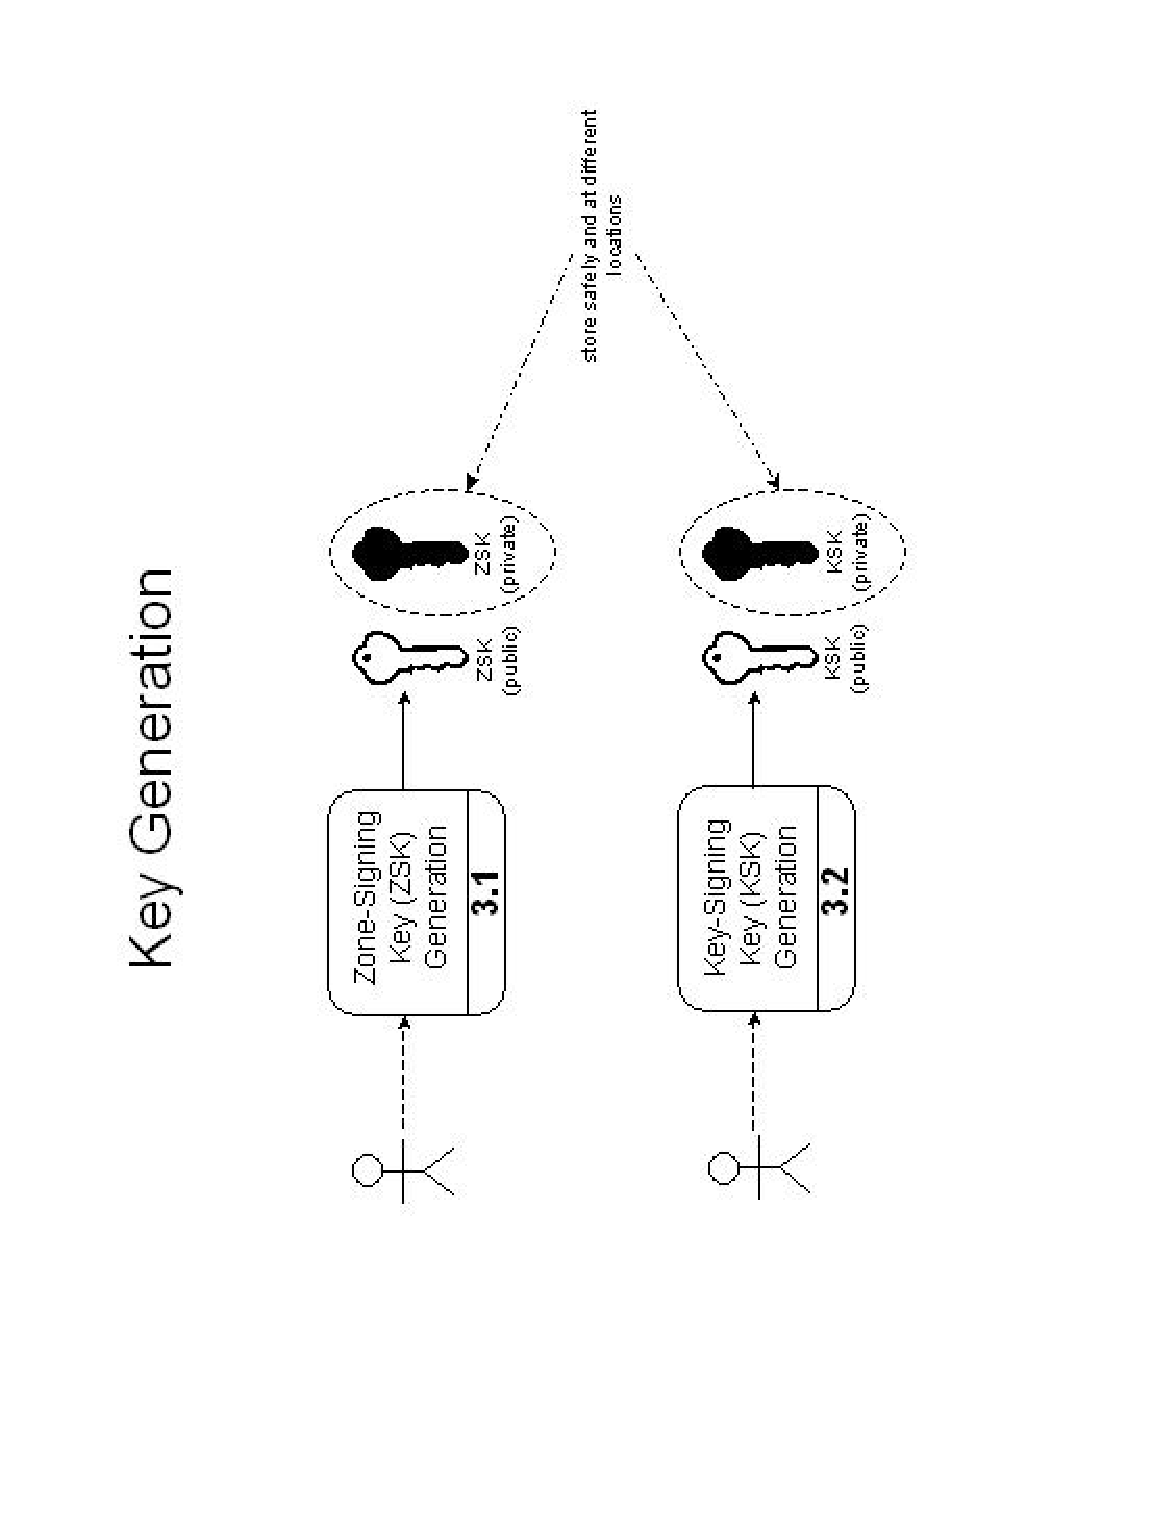
\includegraphics{figure-keygen.ps}
\end{center}
\caption{Key Generation}
\label{fig:keygen}
\end{figure}

\clearpage

\begin{figure}[htb]
\begin{center}
% \leavevmode 
\epsfxsize 6.0in
\epsffile{figure-zskroll.ps}
\end{center}
\caption{ZSK Roll-Over}
\label{fig:zskroll}
\end{figure}

\clearpage

\begin{figure}[htb]
\begin{center}
% \leavevmode 
\epsfxsize 6.0in
\epsffile{figure-kskroll.ps}
\end{center}
\caption{KSK Roll-Over}
\label{fig:kskroll}
\end{figure}

\clearpage

\begin{figure}[htb]
\begin{center}
% \leavevmode 
\epsfxsize 6.0in
\epsffile{figure-securingdeleg-child.ps}
\end{center}
\caption{Securing Delegations -- Child-Zone Activity}
\label{fig:securingdeleg-child}
\end{figure}

\clearpage

\begin{figure}[htb]
\begin{center}
% \leavevmode 
\epsfxsize 6.0in
\epsffile{figure-zonesign-unsecure.ps}
\end{center}
\caption{Zone-Signing with Unsecured Child Delegations}
\label{fig:zonesign-unsecure}
\end{figure}

\clearpage

\begin{figure}[htb]
\begin{center}
% \leavevmode 
\epsfxsize 6.0in
\epsffile{figure-zonesign-secure.ps}
\end{center}
\caption{Zone-Signing with Secured Child Delegations}
\label{fig:zonesign-secure}
\end{figure}

\clearpage

\begin{figure}[htb]
\begin{center}
% \leavevmode 
\epsfxsize 6.0in
\epsffile{figure-securingdeleg-parent.ps}
\end{center}
\caption{Securing Delegations -- Parent-Zone Activity}
\label{fig:securingdeleg-parent}
\end{figure}

\clearpage

\begin{figure}[htb]
\begin{center}
% \leavevmode 
\epsfxsize 6.0in
\epsffile{figure-kskroll-emerg.ps}
\end{center}
\caption{Emergency KSK Roll-Over}
\label{fig:kskroll-emerg}
\end{figure}

\clearpage

\begin{figure}[htb]
\begin{center}
% \leavevmode 
\epsfxsize 6.0in
\epsffile{figure-zskroll-emerg.ps}
\end{center}
\caption{Emergency ZSK Roll-Over}
\label{fig:zskroll-emerg}
\end{figure}

%%%%%%%%%%%%%%%%%%%%%%%%%%%%%%%%%%%%%%

\clearpage

\markboth{Step-by-Step DNS Security Operator Guidance Document - version 0.5}{Step-by-Step DNS Security Operator Guidance Document - version 0.5}
\section{References}
\markboth{Step-by-Step DNS Security Operator Guidance Document - version 0.5}{Step-by-Step DNS Security Operator Guidance Document - version 0.5}
\label{app-refs}

\begin{description}
\item $[$1$]$ O. Kolkman, R. Gieben, ``DNSSEC Operational Practices'',
{\it draft-\-ietf-\-dnsop-\-dnssec-\-operational-\-practices-\-03}
(work in progress), Dec. 23, 2004.

% \item $[$2$]$ {\it TBD (2.1 about randomness)}
% \item $[$3$]$ {\bf there is no reference 3}
% \item $[$4$]$ {\it TBD (intro, discussion of DNSSEC and BIND)}
% \item $[$5$]$ {\it TBD (intro, good intro to DNSSEC)}
% \item $[$6$]$ {\it TBD (2.1 about pseudorandom numbers)}
% \item $[$7$]$ {\it TBD (intro, basic understanding of public key crypto needed)}

\end{description}

\markboth{Step-by-Step DNS Security Operator Guidance Document - version 0.5}{Step-by-Step DNS Security Operator Guidance Document - version 0.5}

%%%%%%%%%%%%%%%%%%%%%%%%%%%%%%%%%%%%%%

\end{document}
